\documentclass[twoside]{book}

% Packages required by doxygen
\usepackage{fixltx2e}
\usepackage{calc}
\usepackage{doxygen}
\usepackage[export]{adjustbox} % also loads graphicx
\usepackage{graphicx}
\usepackage[utf8]{inputenc}
\usepackage{makeidx}
\usepackage{multicol}
\usepackage{multirow}
\PassOptionsToPackage{warn}{textcomp}
\usepackage{textcomp}
\usepackage[nointegrals]{wasysym}
\usepackage[table]{xcolor}

% Font selection
\usepackage[T1]{fontenc}
\usepackage[scaled=.90]{helvet}
\usepackage{courier}
\usepackage{amssymb}
\usepackage{sectsty}
\renewcommand{\familydefault}{\sfdefault}
\allsectionsfont{%
  \fontseries{bc}\selectfont%
  \color{darkgray}%
}
\renewcommand{\DoxyLabelFont}{%
  \fontseries{bc}\selectfont%
  \color{darkgray}%
}
\newcommand{\+}{\discretionary{\mbox{\scriptsize$\hookleftarrow$}}{}{}}

% Page & text layout
\usepackage{geometry}
\geometry{%
  a4paper,%
  top=2.5cm,%
  bottom=2.5cm,%
  left=2.5cm,%
  right=2.5cm%
}
\tolerance=750
\hfuzz=15pt
\hbadness=750
\setlength{\emergencystretch}{15pt}
\setlength{\parindent}{0cm}
\setlength{\parskip}{3ex plus 2ex minus 2ex}
\makeatletter
\renewcommand{\paragraph}{%
  \@startsection{paragraph}{4}{0ex}{-1.0ex}{1.0ex}{%
    \normalfont\normalsize\bfseries\SS@parafont%
  }%
}
\renewcommand{\subparagraph}{%
  \@startsection{subparagraph}{5}{0ex}{-1.0ex}{1.0ex}{%
    \normalfont\normalsize\bfseries\SS@subparafont%
  }%
}
\makeatother

% Headers & footers
\usepackage{fancyhdr}
\pagestyle{fancyplain}
\fancyhead[LE]{\fancyplain{}{\bfseries\thepage}}
\fancyhead[CE]{\fancyplain{}{}}
\fancyhead[RE]{\fancyplain{}{\bfseries\leftmark}}
\fancyhead[LO]{\fancyplain{}{\bfseries\rightmark}}
\fancyhead[CO]{\fancyplain{}{}}
\fancyhead[RO]{\fancyplain{}{\bfseries\thepage}}
\fancyfoot[LE]{\fancyplain{}{}}
\fancyfoot[CE]{\fancyplain{}{}}
\fancyfoot[RE]{\fancyplain{}{\bfseries\scriptsize Generated by Doxygen }}
\fancyfoot[LO]{\fancyplain{}{\bfseries\scriptsize Generated by Doxygen }}
\fancyfoot[CO]{\fancyplain{}{}}
\fancyfoot[RO]{\fancyplain{}{}}
\renewcommand{\footrulewidth}{0.4pt}
\renewcommand{\chaptermark}[1]{%
  \markboth{#1}{}%
}
\renewcommand{\sectionmark}[1]{%
  \markright{\thesection\ #1}%
}

% Indices & bibliography
\usepackage{natbib}
\usepackage[titles]{tocloft}
\setcounter{tocdepth}{3}
\setcounter{secnumdepth}{5}
\makeindex

% Hyperlinks (required, but should be loaded last)
\usepackage{ifpdf}
\ifpdf
  \usepackage[pdftex,pagebackref=true]{hyperref}
\else
  \usepackage[ps2pdf,pagebackref=true]{hyperref}
\fi
\hypersetup{%
  colorlinks=true,%
  linkcolor=blue,%
  citecolor=blue,%
  unicode%
}

% Custom commands
\newcommand{\clearemptydoublepage}{%
  \newpage{\pagestyle{empty}\cleardoublepage}%
}

\usepackage{caption}
\captionsetup{labelsep=space,justification=centering,font={bf},singlelinecheck=off,skip=4pt,position=top}

%===== C O N T E N T S =====

\begin{document}

% Titlepage & ToC
\hypersetup{pageanchor=false,
             bookmarksnumbered=true,
             pdfencoding=unicode
            }
\pagenumbering{alph}
\begin{titlepage}
\vspace*{7cm}
\begin{center}%
{\Large Virtual\+Eye }\\
\vspace*{1cm}
{\large Generated by Doxygen 1.8.12}\\
\end{center}
\end{titlepage}
\clearemptydoublepage
\pagenumbering{roman}
\tableofcontents
\clearemptydoublepage
\pagenumbering{arabic}
\hypersetup{pageanchor=true}

%--- Begin generated contents ---
\chapter{Hierarchical Index}
\section{Class Hierarchy}
This inheritance list is sorted roughly, but not completely, alphabetically\+:\begin{DoxyCompactList}
\item \contentsline{section}{Virtual\+:\+:Camera}{\pageref{class_virtual_1_1_camera}}{}
\item \contentsline{section}{Virtual\+:\+:Clock}{\pageref{class_virtual_1_1_clock}}{}
\item \contentsline{section}{Virtual\+:\+:Color}{\pageref{struct_virtual_1_1_color}}{}
\item \contentsline{section}{Virtual\+:\+:Debug\+Log}{\pageref{class_virtual_1_1_debug_log}}{}
\item \contentsline{section}{Virtual\+:\+:Device}{\pageref{class_virtual_1_1_device}}{}
\item \contentsline{section}{Virtual\+:\+:Drawable}{\pageref{class_virtual_1_1_drawable}}{}
\begin{DoxyCompactList}
\item \contentsline{section}{Virtual\+:\+:Label}{\pageref{class_virtual_1_1_label}}{}
\item \contentsline{section}{Virtual\+:\+:Sprite}{\pageref{class_virtual_1_1_sprite}}{}
\item \contentsline{section}{Virtual\+:\+:Tile}{\pageref{class_virtual_1_1_tile}}{}
\end{DoxyCompactList}
\item \contentsline{section}{Virtual\+:\+:Event\+Manager}{\pageref{class_virtual_1_1_event_manager}}{}
\item \contentsline{section}{Virtual\+:\+:Font}{\pageref{class_virtual_1_1_font}}{}
\item \contentsline{section}{Virtual\+:\+:Map}{\pageref{struct_virtual_1_1_map}}{}
\item \contentsline{section}{Virtual\+:\+:Music\+Player}{\pageref{class_virtual_1_1_music_player}}{}
\item \contentsline{section}{Virtual\+:\+:Name\+Object}{\pageref{class_virtual_1_1_name_object}}{}
\begin{DoxyCompactList}
\item \contentsline{section}{Virtual\+:\+:Label}{\pageref{class_virtual_1_1_label}}{}
\item \contentsline{section}{Virtual\+:\+:Music}{\pageref{class_virtual_1_1_music}}{}
\item \contentsline{section}{Virtual\+:\+:Sprite}{\pageref{class_virtual_1_1_sprite}}{}
\item \contentsline{section}{Virtual\+:\+:Tile}{\pageref{class_virtual_1_1_tile}}{}
\end{DoxyCompactList}
\item \contentsline{section}{Virtual\+:\+:Rectangle$<$ T $>$}{\pageref{struct_virtual_1_1_rectangle}}{}
\item \contentsline{section}{Virtual\+:\+:Renderer}{\pageref{class_virtual_1_1_renderer}}{}
\item \contentsline{section}{Virtual\+:\+:Texture}{\pageref{class_virtual_1_1_texture}}{}
\begin{DoxyCompactList}
\item \contentsline{section}{Virtual\+:\+:Label}{\pageref{class_virtual_1_1_label}}{}
\item \contentsline{section}{Virtual\+:\+:Sprite}{\pageref{class_virtual_1_1_sprite}}{}
\item \contentsline{section}{Virtual\+:\+:Tile}{\pageref{class_virtual_1_1_tile}}{}
\end{DoxyCompactList}
\item \contentsline{section}{Virtual\+:\+:Transformable}{\pageref{class_virtual_1_1_transformable}}{}
\begin{DoxyCompactList}
\item \contentsline{section}{Virtual\+:\+:Label}{\pageref{class_virtual_1_1_label}}{}
\item \contentsline{section}{Virtual\+:\+:Sprite}{\pageref{class_virtual_1_1_sprite}}{}
\item \contentsline{section}{Virtual\+:\+:Tile}{\pageref{class_virtual_1_1_tile}}{}
\end{DoxyCompactList}
\item \contentsline{section}{Virtual\+:\+:Vector2$<$ T $>$}{\pageref{struct_virtual_1_1_vector2}}{}
\item \contentsline{section}{Virtual\+:\+:Vector2$<$ int $>$}{\pageref{struct_virtual_1_1_vector2}}{}
\end{DoxyCompactList}

\chapter{Class Index}
\section{Class List}
Here are the classes, structs, unions and interfaces with brief descriptions\+:\begin{DoxyCompactList}
\item\contentsline{section}{\hyperlink{class_virtual_1_1_camera}{Virtual\+::\+Camera} \\*Just camera }{\pageref{class_virtual_1_1_camera}}{}
\item\contentsline{section}{\hyperlink{class_virtual_1_1_clock}{Virtual\+::\+Clock} \\*Managment of time }{\pageref{class_virtual_1_1_clock}}{}
\item\contentsline{section}{\hyperlink{struct_virtual_1_1_color}{Virtual\+::\+Color} \\*The simple structure of R\+GB \hyperlink{struct_virtual_1_1_color}{Color} }{\pageref{struct_virtual_1_1_color}}{}
\item\contentsline{section}{\hyperlink{class_virtual_1_1_debug_log}{Virtual\+::\+Debug\+Log} \\*Singleton to manage debugging }{\pageref{class_virtual_1_1_debug_log}}{}
\item\contentsline{section}{\hyperlink{class_virtual_1_1_device}{Virtual\+::\+Device} \\*Managment of sublibraries, window and all of the classes of engine }{\pageref{class_virtual_1_1_device}}{}
\item\contentsline{section}{\hyperlink{class_virtual_1_1_drawable}{Virtual\+::\+Drawable} \\*Class able to drawing by engine }{\pageref{class_virtual_1_1_drawable}}{}
\item\contentsline{section}{\hyperlink{class_virtual_1_1_event_manager}{Virtual\+::\+Event\+Manager} \\*Management of event queque }{\pageref{class_virtual_1_1_event_manager}}{}
\item\contentsline{section}{\hyperlink{class_virtual_1_1_font}{Virtual\+::\+Font} \\*Simple font dynamic class, like \hyperlink{class_virtual_1_1_texture}{Texture} }{\pageref{class_virtual_1_1_font}}{}
\item\contentsline{section}{\hyperlink{class_virtual_1_1_label}{Virtual\+::\+Label} \\*Simple sprite dynamic class, like \hyperlink{class_virtual_1_1_sprite}{Sprite} }{\pageref{class_virtual_1_1_label}}{}
\item\contentsline{section}{\hyperlink{struct_virtual_1_1_map}{Virtual\+::\+Map} \\*Info about map }{\pageref{struct_virtual_1_1_map}}{}
\item\contentsline{section}{\hyperlink{class_virtual_1_1_music}{Virtual\+::\+Music} }{\pageref{class_virtual_1_1_music}}{}
\item\contentsline{section}{\hyperlink{class_virtual_1_1_music_player}{Virtual\+::\+Music\+Player} \\*Class to play music }{\pageref{class_virtual_1_1_music_player}}{}
\item\contentsline{section}{\hyperlink{class_virtual_1_1_name_object}{Virtual\+::\+Name\+Object} }{\pageref{class_virtual_1_1_name_object}}{}
\item\contentsline{section}{\hyperlink{struct_virtual_1_1_rectangle}{Virtual\+::\+Rectangle$<$ T $>$} \\*The simple coorinates of \hyperlink{struct_virtual_1_1_rectangle}{Rectangle} }{\pageref{struct_virtual_1_1_rectangle}}{}
\item\contentsline{section}{\hyperlink{class_virtual_1_1_renderer}{Virtual\+::\+Renderer} \\*Management of current scene }{\pageref{class_virtual_1_1_renderer}}{}
\item\contentsline{section}{\hyperlink{class_virtual_1_1_sprite}{Virtual\+::\+Sprite} \\*Simple sprite class, like \hyperlink{class_virtual_1_1_label}{Label} }{\pageref{class_virtual_1_1_sprite}}{}
\item\contentsline{section}{\hyperlink{class_virtual_1_1_texture}{Virtual\+::\+Texture} \\*Dynamic texture class, like \hyperlink{class_virtual_1_1_font}{Font} }{\pageref{class_virtual_1_1_texture}}{}
\item\contentsline{section}{\hyperlink{class_virtual_1_1_tile}{Virtual\+::\+Tile} \\*Simple tile class }{\pageref{class_virtual_1_1_tile}}{}
\item\contentsline{section}{\hyperlink{class_virtual_1_1_transformable}{Virtual\+::\+Transformable} \\*Class to manupulate position and size of object }{\pageref{class_virtual_1_1_transformable}}{}
\item\contentsline{section}{\hyperlink{struct_virtual_1_1_vector2}{Virtual\+::\+Vector2$<$ T $>$} \\*The simple coorinates of one point on the screen }{\pageref{struct_virtual_1_1_vector2}}{}
\end{DoxyCompactList}

\chapter{Class Documentation}
\hypertarget{class_virtual_1_1_camera}{}\section{Virtual\+:\+:Camera Class Reference}
\label{class_virtual_1_1_camera}\index{Virtual\+::\+Camera@{Virtual\+::\+Camera}}


Just camera.  




{\ttfamily \#include $<$Camera.\+hpp$>$}

\subsection*{Public Member Functions}
\begin{DoxyCompactItemize}
\item 
void \hyperlink{class_virtual_1_1_camera_a6916239ab1b8ad4a9b1c20c36f28de18}{update} (\hyperlink{struct_virtual_1_1_vector2}{Vector2}$<$ int $>$ window\+Resolution, \hyperlink{struct_virtual_1_1_vector2}{Vector2}$<$ int $>$ level\+Resolution)
\begin{DoxyCompactList}\small\item\em Updates the info about resolution of window and level. \end{DoxyCompactList}\item 
void \hyperlink{class_virtual_1_1_camera_ae6c71fea6b4f46be3af9c015507576a0}{set\+Center} (\hyperlink{struct_virtual_1_1_vector2}{Vector2}$<$ int $>$ center\+Position)
\begin{DoxyCompactList}\small\item\em Updates position of camera. \end{DoxyCompactList}\item 
void \hyperlink{class_virtual_1_1_camera_ac6ec60ab0905c4ddcaa835914d20f770}{move} (\hyperlink{struct_virtual_1_1_vector2}{Vector2}$<$ int $>$ relative\+Position)
\begin{DoxyCompactList}\small\item\em Move the camera relativly of previous position. \end{DoxyCompactList}\item 
S\+D\+L\+\_\+\+Rect \hyperlink{class_virtual_1_1_camera_a45d86b427fa74b7c0bf2febe1d20cb01}{get\+Rect} ()
\end{DoxyCompactItemize}


\subsection{Detailed Description}
Just camera. 

\subsection{Member Function Documentation}
\hypertarget{class_virtual_1_1_camera_a45d86b427fa74b7c0bf2febe1d20cb01}{}\label{class_virtual_1_1_camera_a45d86b427fa74b7c0bf2febe1d20cb01} 
\index{Virtual\+::\+Camera@{Virtual\+::\+Camera}!get\+Rect@{get\+Rect}}
\index{get\+Rect@{get\+Rect}!Virtual\+::\+Camera@{Virtual\+::\+Camera}}
\subsubsection{\texorpdfstring{get\+Rect()}{getRect()}}
{\footnotesize\ttfamily S\+D\+L\+\_\+\+Rect Virtual\+::\+Camera\+::get\+Rect (\begin{DoxyParamCaption}{ }\end{DoxyParamCaption})}

\begin{DoxyReturn}{Returns}
S\+DL rectangle of position and resolution of camera 
\end{DoxyReturn}
\hypertarget{class_virtual_1_1_camera_ac6ec60ab0905c4ddcaa835914d20f770}{}\label{class_virtual_1_1_camera_ac6ec60ab0905c4ddcaa835914d20f770} 
\index{Virtual\+::\+Camera@{Virtual\+::\+Camera}!move@{move}}
\index{move@{move}!Virtual\+::\+Camera@{Virtual\+::\+Camera}}
\subsubsection{\texorpdfstring{move()}{move()}}
{\footnotesize\ttfamily void Virtual\+::\+Camera\+::move (\begin{DoxyParamCaption}\item[{\hyperlink{struct_virtual_1_1_vector2}{Vector2}$<$ int $>$}]{relative\+Position }\end{DoxyParamCaption})}



Move the camera relativly of previous position. 


\begin{DoxyParams}{Parameters}
{\em relative\+Position} & -\/ Integer vector of changed position \\
\hline
\end{DoxyParams}
\hypertarget{class_virtual_1_1_camera_ae6c71fea6b4f46be3af9c015507576a0}{}\label{class_virtual_1_1_camera_ae6c71fea6b4f46be3af9c015507576a0} 
\index{Virtual\+::\+Camera@{Virtual\+::\+Camera}!set\+Center@{set\+Center}}
\index{set\+Center@{set\+Center}!Virtual\+::\+Camera@{Virtual\+::\+Camera}}
\subsubsection{\texorpdfstring{set\+Center()}{setCenter()}}
{\footnotesize\ttfamily void Virtual\+::\+Camera\+::set\+Center (\begin{DoxyParamCaption}\item[{\hyperlink{struct_virtual_1_1_vector2}{Vector2}$<$ int $>$}]{center\+Position }\end{DoxyParamCaption})}



Updates position of camera. 


\begin{DoxyParams}{Parameters}
{\em center\+Position} & -\/ Integer vector of center of camera \\
\hline
\end{DoxyParams}
\hypertarget{class_virtual_1_1_camera_a6916239ab1b8ad4a9b1c20c36f28de18}{}\label{class_virtual_1_1_camera_a6916239ab1b8ad4a9b1c20c36f28de18} 
\index{Virtual\+::\+Camera@{Virtual\+::\+Camera}!update@{update}}
\index{update@{update}!Virtual\+::\+Camera@{Virtual\+::\+Camera}}
\subsubsection{\texorpdfstring{update()}{update()}}
{\footnotesize\ttfamily void Virtual\+::\+Camera\+::update (\begin{DoxyParamCaption}\item[{\hyperlink{struct_virtual_1_1_vector2}{Vector2}$<$ int $>$}]{window\+Resolution,  }\item[{\hyperlink{struct_virtual_1_1_vector2}{Vector2}$<$ int $>$}]{level\+Resolution }\end{DoxyParamCaption})}



Updates the info about resolution of window and level. 


\begin{DoxyParams}{Parameters}
{\em window\+Resolution} & -\/ Integer vectors of resolution of window \\
\hline
{\em level\+Resolution} & -\/ Integer vectors of resolution of map \\
\hline
\end{DoxyParams}


The documentation for this class was generated from the following file\+:\begin{DoxyCompactItemize}
\item 
include/\+Virtual\+Eye/Camera.\+hpp\end{DoxyCompactItemize}

\hypertarget{class_virtual_1_1_clock}{}\section{Virtual\+:\+:Clock Class Reference}
\label{class_virtual_1_1_clock}\index{Virtual\+::\+Clock@{Virtual\+::\+Clock}}


Managment of time.  




{\ttfamily \#include $<$Clock.\+hpp$>$}

\subsection*{Public Member Functions}
\begin{DoxyCompactItemize}
\item 
\hypertarget{class_virtual_1_1_clock_afadf22f33ce39602ec633dea45ea5071}{}\label{class_virtual_1_1_clock_afadf22f33ce39602ec633dea45ea5071} 
void \hyperlink{class_virtual_1_1_clock_afadf22f33ce39602ec633dea45ea5071}{start} (void)
\begin{DoxyCompactList}\small\item\em Start of the time catching. \end{DoxyCompactList}\item 
\hypertarget{class_virtual_1_1_clock_a7a32ac32a06ef34178d985b0a6c08c57}{}\label{class_virtual_1_1_clock_a7a32ac32a06ef34178d985b0a6c08c57} 
void \hyperlink{class_virtual_1_1_clock_a7a32ac32a06ef34178d985b0a6c08c57}{stop} (void)
\begin{DoxyCompactList}\small\item\em Catching, calculating the time. \end{DoxyCompactList}\item 
double \hyperlink{class_virtual_1_1_clock_a93eb30323793a30b8fd0afee4389d471}{get\+Delta} (void)
\end{DoxyCompactItemize}


\subsection{Detailed Description}
Managment of time. 

\subsection{Member Function Documentation}
\hypertarget{class_virtual_1_1_clock_a93eb30323793a30b8fd0afee4389d471}{}\label{class_virtual_1_1_clock_a93eb30323793a30b8fd0afee4389d471} 
\index{Virtual\+::\+Clock@{Virtual\+::\+Clock}!get\+Delta@{get\+Delta}}
\index{get\+Delta@{get\+Delta}!Virtual\+::\+Clock@{Virtual\+::\+Clock}}
\subsubsection{\texorpdfstring{get\+Delta()}{getDelta()}}
{\footnotesize\ttfamily double Virtual\+::\+Clock\+::get\+Delta (\begin{DoxyParamCaption}\item[{void}]{ }\end{DoxyParamCaption})}

\begin{DoxyReturn}{Returns}
In-\/double odd of the start and stop time 
\end{DoxyReturn}


The documentation for this class was generated from the following file\+:\begin{DoxyCompactItemize}
\item 
include/\+Virtual\+Eye/Clock.\+hpp\end{DoxyCompactItemize}

\hypertarget{struct_virtual_1_1_color}{}\section{Virtual\+:\+:Color Struct Reference}
\label{struct_virtual_1_1_color}\index{Virtual\+::\+Color@{Virtual\+::\+Color}}


The simple structure of R\+GB \hyperlink{struct_virtual_1_1_color}{Color}.  




{\ttfamily \#include $<$Math.\+hpp$>$}

\subsection*{Public Member Functions}
\begin{DoxyCompactItemize}
\item 
\hyperlink{struct_virtual_1_1_color_a003277f5a30952ecccedbb61ad347ddc}{Color} ()
\begin{DoxyCompactList}\small\item\em Default 255 constructor. \end{DoxyCompactList}\item 
\hyperlink{struct_virtual_1_1_color_a04237a9e45fdf6378288d5b93573ace7}{Color} (float rr, float gg, float bb)
\begin{DoxyCompactList}\small\item\em Default custom constructor. \end{DoxyCompactList}\end{DoxyCompactItemize}
\subsection*{Public Attributes}
\begin{DoxyCompactItemize}
\item 
\hypertarget{struct_virtual_1_1_color_afc2067553aabb70f0b84a8e36793f1a1}{}\label{struct_virtual_1_1_color_afc2067553aabb70f0b84a8e36793f1a1} 
Uint8 {\bfseries r}
\item 
\hypertarget{struct_virtual_1_1_color_a2966b2965d8be251c3c9d0f4f428f857}{}\label{struct_virtual_1_1_color_a2966b2965d8be251c3c9d0f4f428f857} 
Uint8 {\bfseries g}
\item 
\hypertarget{struct_virtual_1_1_color_a3aaa995ed8089d50d039783f7e6c8b03}{}\label{struct_virtual_1_1_color_a3aaa995ed8089d50d039783f7e6c8b03} 
Uint8 {\bfseries b}
\end{DoxyCompactItemize}


\subsection{Detailed Description}
The simple structure of R\+GB \hyperlink{struct_virtual_1_1_color}{Color}. 

\subsection{Constructor \& Destructor Documentation}
\hypertarget{struct_virtual_1_1_color_a003277f5a30952ecccedbb61ad347ddc}{}\label{struct_virtual_1_1_color_a003277f5a30952ecccedbb61ad347ddc} 
\index{Virtual\+::\+Color@{Virtual\+::\+Color}!Color@{Color}}
\index{Color@{Color}!Virtual\+::\+Color@{Virtual\+::\+Color}}
\subsubsection{\texorpdfstring{Color()}{Color()}\hspace{0.1cm}{\footnotesize\ttfamily [1/2]}}
{\footnotesize\ttfamily Virtual\+::\+Color\+::\+Color (\begin{DoxyParamCaption}{ }\end{DoxyParamCaption})\hspace{0.3cm}{\ttfamily [inline]}}



Default 255 constructor. 

This constructor append of each variables 255. \hypertarget{struct_virtual_1_1_color_a04237a9e45fdf6378288d5b93573ace7}{}\label{struct_virtual_1_1_color_a04237a9e45fdf6378288d5b93573ace7} 
\index{Virtual\+::\+Color@{Virtual\+::\+Color}!Color@{Color}}
\index{Color@{Color}!Virtual\+::\+Color@{Virtual\+::\+Color}}
\subsubsection{\texorpdfstring{Color()}{Color()}\hspace{0.1cm}{\footnotesize\ttfamily [2/2]}}
{\footnotesize\ttfamily Virtual\+::\+Color\+::\+Color (\begin{DoxyParamCaption}\item[{float}]{rr,  }\item[{float}]{gg,  }\item[{float}]{bb }\end{DoxyParamCaption})\hspace{0.3cm}{\ttfamily [inline]}}



Default custom constructor. 


\begin{DoxyParams}{Parameters}
{\em rr} & -\/ red intensity of color \\
\hline
{\em gg} & -\/ gren intensity of color \\
\hline
{\em bb} & -\/ blue intensity of color\\
\hline
\end{DoxyParams}
This constructor append of each variables given values. 

The documentation for this struct was generated from the following file\+:\begin{DoxyCompactItemize}
\item 
include/\+Virtual\+Eye/Math.\+hpp\end{DoxyCompactItemize}

\hypertarget{class_virtual_1_1_debug_log}{}\section{Virtual\+:\+:Debug\+Log Class Reference}
\label{class_virtual_1_1_debug_log}\index{Virtual\+::\+Debug\+Log@{Virtual\+::\+Debug\+Log}}


Singleton to manage debugging.  




{\ttfamily \#include $<$Debug\+Log.\+hpp$>$}

\subsection*{Public Member Functions}
\begin{DoxyCompactItemize}
\item 
void \hyperlink{class_virtual_1_1_debug_log_af629e3c39eb80538b8b62076fb02ad4b}{add\+To\+Log} (std\+::string string)
\begin{DoxyCompactList}\small\item\em Adds the string into log. \end{DoxyCompactList}\item 
\hypertarget{class_virtual_1_1_debug_log_ab272eb11cbba0e95cb4df862667c112b}{}\label{class_virtual_1_1_debug_log_ab272eb11cbba0e95cb4df862667c112b} 
void \hyperlink{class_virtual_1_1_debug_log_ab272eb11cbba0e95cb4df862667c112b}{print\+Log} ()
\begin{DoxyCompactList}\small\item\em create debug log file and print to they all logs \end{DoxyCompactList}\end{DoxyCompactItemize}
\subsection*{Static Public Member Functions}
\begin{DoxyCompactItemize}
\item 
static \hyperlink{class_virtual_1_1_debug_log}{Debug\+Log} \& \hyperlink{class_virtual_1_1_debug_log_a7360c164a4fa8df9a68449bdf4c38ecf}{get\+Instance} ()
\end{DoxyCompactItemize}


\subsection{Detailed Description}
Singleton to manage debugging. 

\subsection{Member Function Documentation}
\hypertarget{class_virtual_1_1_debug_log_af629e3c39eb80538b8b62076fb02ad4b}{}\label{class_virtual_1_1_debug_log_af629e3c39eb80538b8b62076fb02ad4b} 
\index{Virtual\+::\+Debug\+Log@{Virtual\+::\+Debug\+Log}!add\+To\+Log@{add\+To\+Log}}
\index{add\+To\+Log@{add\+To\+Log}!Virtual\+::\+Debug\+Log@{Virtual\+::\+Debug\+Log}}
\subsubsection{\texorpdfstring{add\+To\+Log()}{addToLog()}}
{\footnotesize\ttfamily void Virtual\+::\+Debug\+Log\+::add\+To\+Log (\begin{DoxyParamCaption}\item[{std\+::string}]{string }\end{DoxyParamCaption})}



Adds the string into log. 


\begin{DoxyParams}{Parameters}
{\em string} & -\/ Value that want to print into debug log \\
\hline
\end{DoxyParams}
\hypertarget{class_virtual_1_1_debug_log_a7360c164a4fa8df9a68449bdf4c38ecf}{}\label{class_virtual_1_1_debug_log_a7360c164a4fa8df9a68449bdf4c38ecf} 
\index{Virtual\+::\+Debug\+Log@{Virtual\+::\+Debug\+Log}!get\+Instance@{get\+Instance}}
\index{get\+Instance@{get\+Instance}!Virtual\+::\+Debug\+Log@{Virtual\+::\+Debug\+Log}}
\subsubsection{\texorpdfstring{get\+Instance()}{getInstance()}}
{\footnotesize\ttfamily static \hyperlink{class_virtual_1_1_debug_log}{Debug\+Log}\& Virtual\+::\+Debug\+Log\+::get\+Instance (\begin{DoxyParamCaption}{ }\end{DoxyParamCaption})\hspace{0.3cm}{\ttfamily [static]}}

\begin{DoxyReturn}{Returns}
instance to singleton 
\end{DoxyReturn}


The documentation for this class was generated from the following file\+:\begin{DoxyCompactItemize}
\item 
include/\+Virtual\+Eye/Debug\+Log.\+hpp\end{DoxyCompactItemize}

\hypertarget{class_virtual_1_1_device}{}\section{Virtual\+:\+:Device Class Reference}
\label{class_virtual_1_1_device}\index{Virtual\+::\+Device@{Virtual\+::\+Device}}


Managment of sublibraries, window and all of the classes of engine.  




{\ttfamily \#include $<$Device.\+hpp$>$}

\subsection*{Public Member Functions}
\begin{DoxyCompactItemize}
\item 
\hyperlink{class_virtual_1_1_device_a01750717800affee98304503b6e7394d}{Device} (int width, int height)
\begin{DoxyCompactList}\small\item\em Init of window, all sublibs and all of the subclasses. \end{DoxyCompactList}\item 
int \hyperlink{class_virtual_1_1_device_aaadbfd2dd970af7a42a858ee52d36869}{start} (std\+::string path)
\begin{DoxyCompactList}\small\item\em Starting the work of game engine, run of all scripts. \end{DoxyCompactList}\end{DoxyCompactItemize}
\subsection*{Protected Member Functions}
\begin{DoxyCompactItemize}
\item 
\hypertarget{class_virtual_1_1_device_acf167a3fc503db0b87bab4435bfef1ed}{}\label{class_virtual_1_1_device_acf167a3fc503db0b87bab4435bfef1ed} 
virtual void \hyperlink{class_virtual_1_1_device_acf167a3fc503db0b87bab4435bfef1ed}{on\+Init} ()
\begin{DoxyCompactList}\small\item\em This function starts before the main loop. \end{DoxyCompactList}\item 
\hypertarget{class_virtual_1_1_device_abbf3596a61ffc42d8b0a533f07e892a7}{}\label{class_virtual_1_1_device_abbf3596a61ffc42d8b0a533f07e892a7} 
virtual void \hyperlink{class_virtual_1_1_device_abbf3596a61ffc42d8b0a533f07e892a7}{on\+Update} ()
\begin{DoxyCompactList}\small\item\em This function starts in the main loop. \end{DoxyCompactList}\item 
void \hyperlink{class_virtual_1_1_device_a15e199ed381e9cf1eea79ce2da30786e}{set\+Parametres} (\hyperlink{struct_virtual_1_1_vector2}{Vector2}$<$ int $>$ resolution)
\begin{DoxyCompactList}\small\item\em Starting the work of game engine, run of all scripts. \end{DoxyCompactList}\item 
void \hyperlink{class_virtual_1_1_device_a7f0a80fead7847616b92d0defad43d96}{set\+Full\+Screened} (bool is\+True)
\begin{DoxyCompactList}\small\item\em Setting is the window run in fullscreen mode or not. \end{DoxyCompactList}\end{DoxyCompactItemize}
\subsection*{Protected Attributes}
\begin{DoxyCompactItemize}
\item 
\hypertarget{class_virtual_1_1_device_aa1ea93335ccb046238b1fb61e1cb087f}{}\label{class_virtual_1_1_device_aa1ea93335ccb046238b1fb61e1cb087f} 
std\+::shared\+\_\+ptr$<$ \hyperlink{class_virtual_1_1_event_manager}{Event\+Manager} $>$ {\bfseries event\+Manager}
\item 
\hypertarget{class_virtual_1_1_device_a3c40ddcdd5514b6ceb8de171835aa522}{}\label{class_virtual_1_1_device_a3c40ddcdd5514b6ceb8de171835aa522} 
std\+::shared\+\_\+ptr$<$ \hyperlink{class_virtual_1_1_renderer}{Renderer} $>$ {\bfseries renderer}
\item 
\hypertarget{class_virtual_1_1_device_a34e3c67e5ed6f3aad78e69df09760079}{}\label{class_virtual_1_1_device_a34e3c67e5ed6f3aad78e69df09760079} 
std\+::shared\+\_\+ptr$<$ \hyperlink{class_virtual_1_1_camera}{Camera} $>$ {\bfseries camera}
\item 
\hypertarget{class_virtual_1_1_device_ae791d56234f12d666bc620d740690067}{}\label{class_virtual_1_1_device_ae791d56234f12d666bc620d740690067} 
std\+::shared\+\_\+ptr$<$ \hyperlink{class_virtual_1_1_clock}{Clock} $>$ {\bfseries clock}
\item 
\hypertarget{class_virtual_1_1_device_aa2bf96683fa3d4fec7b1db02e81caa0b}{}\label{class_virtual_1_1_device_aa2bf96683fa3d4fec7b1db02e81caa0b} 
\hyperlink{struct_virtual_1_1_vector2}{Vector2}$<$ int $>$ {\bfseries level\+Properties}
\end{DoxyCompactItemize}


\subsection{Detailed Description}
Managment of sublibraries, window and all of the classes of engine. 

\subsection{Constructor \& Destructor Documentation}
\hypertarget{class_virtual_1_1_device_a01750717800affee98304503b6e7394d}{}\label{class_virtual_1_1_device_a01750717800affee98304503b6e7394d} 
\index{Virtual\+::\+Device@{Virtual\+::\+Device}!Device@{Device}}
\index{Device@{Device}!Virtual\+::\+Device@{Virtual\+::\+Device}}
\subsubsection{\texorpdfstring{Device()}{Device()}}
{\footnotesize\ttfamily Virtual\+::\+Device\+::\+Device (\begin{DoxyParamCaption}\item[{int}]{width,  }\item[{int}]{height }\end{DoxyParamCaption})}



Init of window, all sublibs and all of the subclasses. 


\begin{DoxyParams}{Parameters}
{\em width,height} & -\/ resolution of window \\
\hline
\end{DoxyParams}


\subsection{Member Function Documentation}
\hypertarget{class_virtual_1_1_device_a7f0a80fead7847616b92d0defad43d96}{}\label{class_virtual_1_1_device_a7f0a80fead7847616b92d0defad43d96} 
\index{Virtual\+::\+Device@{Virtual\+::\+Device}!set\+Full\+Screened@{set\+Full\+Screened}}
\index{set\+Full\+Screened@{set\+Full\+Screened}!Virtual\+::\+Device@{Virtual\+::\+Device}}
\subsubsection{\texorpdfstring{set\+Full\+Screened()}{setFullScreened()}}
{\footnotesize\ttfamily void Virtual\+::\+Device\+::set\+Full\+Screened (\begin{DoxyParamCaption}\item[{bool}]{is\+True }\end{DoxyParamCaption})\hspace{0.3cm}{\ttfamily [protected]}}



Setting is the window run in fullscreen mode or not. 


\begin{DoxyParams}{Parameters}
{\em is\+True} & -\/ true to set fullscreen mode, false to unset fullscreen mode \\
\hline
\end{DoxyParams}
\hypertarget{class_virtual_1_1_device_a15e199ed381e9cf1eea79ce2da30786e}{}\label{class_virtual_1_1_device_a15e199ed381e9cf1eea79ce2da30786e} 
\index{Virtual\+::\+Device@{Virtual\+::\+Device}!set\+Parametres@{set\+Parametres}}
\index{set\+Parametres@{set\+Parametres}!Virtual\+::\+Device@{Virtual\+::\+Device}}
\subsubsection{\texorpdfstring{set\+Parametres()}{setParametres()}}
{\footnotesize\ttfamily void Virtual\+::\+Device\+::set\+Parametres (\begin{DoxyParamCaption}\item[{\hyperlink{struct_virtual_1_1_vector2}{Vector2}$<$ int $>$}]{resolution }\end{DoxyParamCaption})\hspace{0.3cm}{\ttfamily [protected]}}



Starting the work of game engine, run of all scripts. 


\begin{DoxyParams}{Parameters}
{\em resolution} & -\/ resolution of window in integer vector \\
\hline
\end{DoxyParams}
\hypertarget{class_virtual_1_1_device_aaadbfd2dd970af7a42a858ee52d36869}{}\label{class_virtual_1_1_device_aaadbfd2dd970af7a42a858ee52d36869} 
\index{Virtual\+::\+Device@{Virtual\+::\+Device}!start@{start}}
\index{start@{start}!Virtual\+::\+Device@{Virtual\+::\+Device}}
\subsubsection{\texorpdfstring{start()}{start()}}
{\footnotesize\ttfamily int Virtual\+::\+Device\+::start (\begin{DoxyParamCaption}\item[{std\+::string}]{path }\end{DoxyParamCaption})}



Starting the work of game engine, run of all scripts. 


\begin{DoxyParams}{Parameters}
{\em path} & -\/ lua script path \\
\hline
\end{DoxyParams}


The documentation for this class was generated from the following file\+:\begin{DoxyCompactItemize}
\item 
include/\+Virtual\+Eye/Device.\+hpp\end{DoxyCompactItemize}

\hypertarget{class_virtual_1_1_drawable}{}\section{Virtual\+:\+:Drawable Class Reference}
\label{class_virtual_1_1_drawable}\index{Virtual\+::\+Drawable@{Virtual\+::\+Drawable}}


Class able to drawing by engine.  




{\ttfamily \#include $<$Render\+Utils.\+hpp$>$}

Inheritance diagram for Virtual\+:\+:Drawable\+:\begin{figure}[H]
\begin{center}
\leavevmode
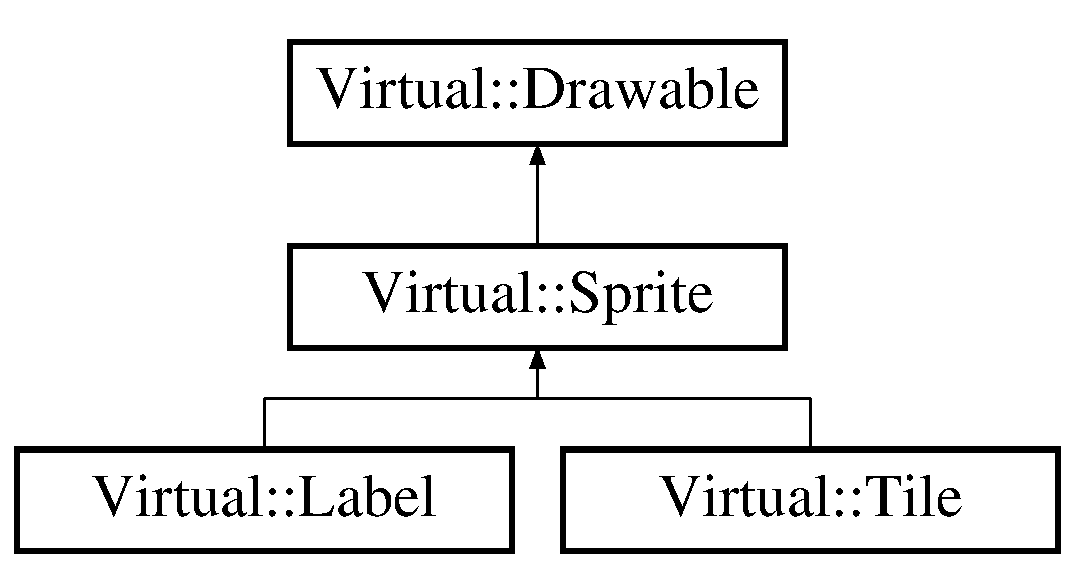
\includegraphics[height=2.000000cm]{class_virtual_1_1_drawable}
\end{center}
\end{figure}
\subsection*{Public Member Functions}
\begin{DoxyCompactItemize}
\item 
virtual void \hyperlink{class_virtual_1_1_drawable_af7014800911efa59b96e538149e56f8b}{draw} (S\+D\+L\+\_\+\+Renderer $\ast$renderer, \hyperlink{class_virtual_1_1_camera}{Camera} \&camera)=0
\begin{DoxyCompactList}\small\item\em Function that use engine to draw object. \end{DoxyCompactList}\item 
bool \hyperlink{class_virtual_1_1_drawable_a7901d5ac8f7ebed5e3d5773c9699ca7c}{is\+Static} ()
\item 
bool \hyperlink{class_virtual_1_1_drawable_a47902855528332fd79595db7dacca2ed}{is\+Drawing} ()
\item 
void \hyperlink{class_virtual_1_1_drawable_a94ed4174ab71aa5aea957d821bc8d170}{set\+Is\+Static} (bool is)
\begin{DoxyCompactList}\small\item\em Sets fact is the object able to be static(don\textquotesingle{}t move by camera) \end{DoxyCompactList}\item 
void \hyperlink{class_virtual_1_1_drawable_af47ef44ac82ef8f11873fcf3e7a4aaa0}{set\+Is\+Drawing} (bool is)
\begin{DoxyCompactList}\small\item\em Sets fact is the object able to drawing by engine. \end{DoxyCompactList}\end{DoxyCompactItemize}
\subsection*{Protected Attributes}
\begin{DoxyCompactItemize}
\item 
\hypertarget{class_virtual_1_1_drawable_a75aa2adddb490011c1efaea42ab16079}{}\label{class_virtual_1_1_drawable_a75aa2adddb490011c1efaea42ab16079} 
bool {\bfseries is\+\_\+static}
\item 
\hypertarget{class_virtual_1_1_drawable_a360d6ddca18c7f4f6699662ba4102c2a}{}\label{class_virtual_1_1_drawable_a360d6ddca18c7f4f6699662ba4102c2a} 
bool {\bfseries is\+\_\+drawing}
\end{DoxyCompactItemize}


\subsection{Detailed Description}
Class able to drawing by engine. 

\subsection{Member Function Documentation}
\hypertarget{class_virtual_1_1_drawable_af7014800911efa59b96e538149e56f8b}{}\label{class_virtual_1_1_drawable_af7014800911efa59b96e538149e56f8b} 
\index{Virtual\+::\+Drawable@{Virtual\+::\+Drawable}!draw@{draw}}
\index{draw@{draw}!Virtual\+::\+Drawable@{Virtual\+::\+Drawable}}
\subsubsection{\texorpdfstring{draw()}{draw()}}
{\footnotesize\ttfamily virtual void Virtual\+::\+Drawable\+::draw (\begin{DoxyParamCaption}\item[{S\+D\+L\+\_\+\+Renderer $\ast$}]{renderer,  }\item[{\hyperlink{class_virtual_1_1_camera}{Camera} \&}]{camera }\end{DoxyParamCaption})\hspace{0.3cm}{\ttfamily [pure virtual]}}



Function that use engine to draw object. 


\begin{DoxyParams}{Parameters}
{\em renderer} & -\/ pointer into S\+D\+L\+\_\+\+Renderer \\
\hline
{\em camera} & -\/ reference to camera in engine \\
\hline
\end{DoxyParams}


Implemented in \hyperlink{class_virtual_1_1_label_aaea754974570ba425d2b9ffe91d183c7}{Virtual\+::\+Label}, \hyperlink{class_virtual_1_1_tile_ac9adb75122a87ec5efb5107b611ba226}{Virtual\+::\+Tile}, and \hyperlink{class_virtual_1_1_sprite_a57f581e0307ab2b2dd7c6922dba2a057}{Virtual\+::\+Sprite}.

\hypertarget{class_virtual_1_1_drawable_a47902855528332fd79595db7dacca2ed}{}\label{class_virtual_1_1_drawable_a47902855528332fd79595db7dacca2ed} 
\index{Virtual\+::\+Drawable@{Virtual\+::\+Drawable}!is\+Drawing@{is\+Drawing}}
\index{is\+Drawing@{is\+Drawing}!Virtual\+::\+Drawable@{Virtual\+::\+Drawable}}
\subsubsection{\texorpdfstring{is\+Drawing()}{isDrawing()}}
{\footnotesize\ttfamily bool Virtual\+::\+Drawable\+::is\+Drawing (\begin{DoxyParamCaption}{ }\end{DoxyParamCaption})}

\begin{DoxyReturn}{Returns}
true if the object was able to drawing / false if it isn\textquotesingle{}t 
\end{DoxyReturn}
\hypertarget{class_virtual_1_1_drawable_a7901d5ac8f7ebed5e3d5773c9699ca7c}{}\label{class_virtual_1_1_drawable_a7901d5ac8f7ebed5e3d5773c9699ca7c} 
\index{Virtual\+::\+Drawable@{Virtual\+::\+Drawable}!is\+Static@{is\+Static}}
\index{is\+Static@{is\+Static}!Virtual\+::\+Drawable@{Virtual\+::\+Drawable}}
\subsubsection{\texorpdfstring{is\+Static()}{isStatic()}}
{\footnotesize\ttfamily bool Virtual\+::\+Drawable\+::is\+Static (\begin{DoxyParamCaption}{ }\end{DoxyParamCaption})}

\begin{DoxyReturn}{Returns}
true if the object was static(doesn\textquotesingle{}t move by camera) / false if it isn\textquotesingle{}t 
\end{DoxyReturn}
\hypertarget{class_virtual_1_1_drawable_af47ef44ac82ef8f11873fcf3e7a4aaa0}{}\label{class_virtual_1_1_drawable_af47ef44ac82ef8f11873fcf3e7a4aaa0} 
\index{Virtual\+::\+Drawable@{Virtual\+::\+Drawable}!set\+Is\+Drawing@{set\+Is\+Drawing}}
\index{set\+Is\+Drawing@{set\+Is\+Drawing}!Virtual\+::\+Drawable@{Virtual\+::\+Drawable}}
\subsubsection{\texorpdfstring{set\+Is\+Drawing()}{setIsDrawing()}}
{\footnotesize\ttfamily void Virtual\+::\+Drawable\+::set\+Is\+Drawing (\begin{DoxyParamCaption}\item[{bool}]{is }\end{DoxyParamCaption})}



Sets fact is the object able to drawing by engine. 


\begin{DoxyParams}{Parameters}
{\em is} & -\/ fact is the object was able to drawing \\
\hline
\end{DoxyParams}
\hypertarget{class_virtual_1_1_drawable_a94ed4174ab71aa5aea957d821bc8d170}{}\label{class_virtual_1_1_drawable_a94ed4174ab71aa5aea957d821bc8d170} 
\index{Virtual\+::\+Drawable@{Virtual\+::\+Drawable}!set\+Is\+Static@{set\+Is\+Static}}
\index{set\+Is\+Static@{set\+Is\+Static}!Virtual\+::\+Drawable@{Virtual\+::\+Drawable}}
\subsubsection{\texorpdfstring{set\+Is\+Static()}{setIsStatic()}}
{\footnotesize\ttfamily void Virtual\+::\+Drawable\+::set\+Is\+Static (\begin{DoxyParamCaption}\item[{bool}]{is }\end{DoxyParamCaption})}



Sets fact is the object able to be static(don\textquotesingle{}t move by camera) 


\begin{DoxyParams}{Parameters}
{\em is} & -\/ fact is the object was static \\
\hline
\end{DoxyParams}


The documentation for this class was generated from the following file\+:\begin{DoxyCompactItemize}
\item 
include/\+Virtual\+Eye/Render\+Utils.\+hpp\end{DoxyCompactItemize}

\hypertarget{class_virtual_1_1_event_manager}{}\section{Virtual\+:\+:Event\+Manager Class Reference}
\label{class_virtual_1_1_event_manager}\index{Virtual\+::\+Event\+Manager@{Virtual\+::\+Event\+Manager}}


Management of event queque.  




{\ttfamily \#include $<$Event\+Manager.\+hpp$>$}

\subsection*{Public Member Functions}
\begin{DoxyCompactItemize}
\item 
bool \hyperlink{class_virtual_1_1_event_manager_ab1f3521b16ff390d968a12c9c8fbc00c}{is\+Closed} (void)
\begin{DoxyCompactList}\small\item\em Check is the window closed. \end{DoxyCompactList}\item 
bool \hyperlink{class_virtual_1_1_event_manager_a565bd5f26862a9f8f102078df1cfa39c}{is\+Key\+Pressed} (int id)
\begin{DoxyCompactList}\small\item\em Check is the keyboard key pressed. \end{DoxyCompactList}\item 
bool \hyperlink{class_virtual_1_1_event_manager_addd617c04422d16843073acc9b8a6d32}{is\+Mouse\+Key\+Pressed} (int id)
\begin{DoxyCompactList}\small\item\em Check is the mouse key pressed. \end{DoxyCompactList}\item 
\hypertarget{class_virtual_1_1_event_manager_a994c1f4c3a9d5af2f7c64cf91900c884}{}\label{class_virtual_1_1_event_manager_a994c1f4c3a9d5af2f7c64cf91900c884} 
void \hyperlink{class_virtual_1_1_event_manager_a994c1f4c3a9d5af2f7c64cf91900c884}{close} (void)
\begin{DoxyCompactList}\small\item\em Colse the window. \end{DoxyCompactList}\item 
int \hyperlink{class_virtual_1_1_event_manager_a2e2394e7bb1ca6c7f2fc45813183d17a}{poll\+Events} (void)
\begin{DoxyCompactList}\small\item\em Polling all events into queque. \end{DoxyCompactList}\item 
\hyperlink{struct_virtual_1_1_vector2}{Vector2}$<$ int $>$ \hyperlink{class_virtual_1_1_event_manager_a3d55fffe71640c02b40788887a1048f0}{get\+Mouse\+Position} (void)
\begin{DoxyCompactList}\small\item\em Catch the mouse position. \end{DoxyCompactList}\end{DoxyCompactItemize}


\subsection{Detailed Description}
Management of event queque. 

\subsection{Member Function Documentation}
\hypertarget{class_virtual_1_1_event_manager_a3d55fffe71640c02b40788887a1048f0}{}\label{class_virtual_1_1_event_manager_a3d55fffe71640c02b40788887a1048f0} 
\index{Virtual\+::\+Event\+Manager@{Virtual\+::\+Event\+Manager}!get\+Mouse\+Position@{get\+Mouse\+Position}}
\index{get\+Mouse\+Position@{get\+Mouse\+Position}!Virtual\+::\+Event\+Manager@{Virtual\+::\+Event\+Manager}}
\subsubsection{\texorpdfstring{get\+Mouse\+Position()}{getMousePosition()}}
{\footnotesize\ttfamily \hyperlink{struct_virtual_1_1_vector2}{Vector2}$<$int$>$ Virtual\+::\+Event\+Manager\+::get\+Mouse\+Position (\begin{DoxyParamCaption}\item[{void}]{ }\end{DoxyParamCaption})}



Catch the mouse position. 

\begin{DoxyReturn}{Returns}
Mouse position relative to window 
\end{DoxyReturn}
\hypertarget{class_virtual_1_1_event_manager_ab1f3521b16ff390d968a12c9c8fbc00c}{}\label{class_virtual_1_1_event_manager_ab1f3521b16ff390d968a12c9c8fbc00c} 
\index{Virtual\+::\+Event\+Manager@{Virtual\+::\+Event\+Manager}!is\+Closed@{is\+Closed}}
\index{is\+Closed@{is\+Closed}!Virtual\+::\+Event\+Manager@{Virtual\+::\+Event\+Manager}}
\subsubsection{\texorpdfstring{is\+Closed()}{isClosed()}}
{\footnotesize\ttfamily bool Virtual\+::\+Event\+Manager\+::is\+Closed (\begin{DoxyParamCaption}\item[{void}]{ }\end{DoxyParamCaption})}



Check is the window closed. 

\begin{DoxyReturn}{Returns}
true if window x button is clicked or false when it isn\textquotesingle{}t 
\end{DoxyReturn}
\hypertarget{class_virtual_1_1_event_manager_a565bd5f26862a9f8f102078df1cfa39c}{}\label{class_virtual_1_1_event_manager_a565bd5f26862a9f8f102078df1cfa39c} 
\index{Virtual\+::\+Event\+Manager@{Virtual\+::\+Event\+Manager}!is\+Key\+Pressed@{is\+Key\+Pressed}}
\index{is\+Key\+Pressed@{is\+Key\+Pressed}!Virtual\+::\+Event\+Manager@{Virtual\+::\+Event\+Manager}}
\subsubsection{\texorpdfstring{is\+Key\+Pressed()}{isKeyPressed()}}
{\footnotesize\ttfamily bool Virtual\+::\+Event\+Manager\+::is\+Key\+Pressed (\begin{DoxyParamCaption}\item[{int}]{id }\end{DoxyParamCaption})}



Check is the keyboard key pressed. 

\begin{DoxyReturn}{Returns}
true if keyboard key pressed is clicked or false when it isn\textquotesingle{}t
\end{DoxyReturn}

\begin{DoxyParams}{Parameters}
{\em id} & -\/ K\+E\+Y(x) where x is the name of key like L\+E\+FT \\
\hline
\end{DoxyParams}
\hypertarget{class_virtual_1_1_event_manager_addd617c04422d16843073acc9b8a6d32}{}\label{class_virtual_1_1_event_manager_addd617c04422d16843073acc9b8a6d32} 
\index{Virtual\+::\+Event\+Manager@{Virtual\+::\+Event\+Manager}!is\+Mouse\+Key\+Pressed@{is\+Mouse\+Key\+Pressed}}
\index{is\+Mouse\+Key\+Pressed@{is\+Mouse\+Key\+Pressed}!Virtual\+::\+Event\+Manager@{Virtual\+::\+Event\+Manager}}
\subsubsection{\texorpdfstring{is\+Mouse\+Key\+Pressed()}{isMouseKeyPressed()}}
{\footnotesize\ttfamily bool Virtual\+::\+Event\+Manager\+::is\+Mouse\+Key\+Pressed (\begin{DoxyParamCaption}\item[{int}]{id }\end{DoxyParamCaption})}



Check is the mouse key pressed. 

\begin{DoxyReturn}{Returns}
true if mouse key pressed is clicked or false when it isn\textquotesingle{}t
\end{DoxyReturn}

\begin{DoxyParams}{Parameters}
{\em id} & -\/ M\+O\+U\+S\+E\+\_\+\+B\+U\+T\+T\+O\+N(x) where x is the name of key like L\+E\+FT \\
\hline
\end{DoxyParams}
\hypertarget{class_virtual_1_1_event_manager_a2e2394e7bb1ca6c7f2fc45813183d17a}{}\label{class_virtual_1_1_event_manager_a2e2394e7bb1ca6c7f2fc45813183d17a} 
\index{Virtual\+::\+Event\+Manager@{Virtual\+::\+Event\+Manager}!poll\+Events@{poll\+Events}}
\index{poll\+Events@{poll\+Events}!Virtual\+::\+Event\+Manager@{Virtual\+::\+Event\+Manager}}
\subsubsection{\texorpdfstring{poll\+Events()}{pollEvents()}}
{\footnotesize\ttfamily int Virtual\+::\+Event\+Manager\+::poll\+Events (\begin{DoxyParamCaption}\item[{void}]{ }\end{DoxyParamCaption})}



Polling all events into queque. 

\begin{DoxyReturn}{Returns}
Number of current event 
\end{DoxyReturn}


The documentation for this class was generated from the following file\+:\begin{DoxyCompactItemize}
\item 
include/\+Virtual\+Eye/Event\+Manager.\+hpp\end{DoxyCompactItemize}

\hypertarget{class_virtual_1_1_font}{}\section{Virtual\+:\+:Font Class Reference}
\label{class_virtual_1_1_font}\index{Virtual\+::\+Font@{Virtual\+::\+Font}}


Simple font dynamic class, like \hyperlink{class_virtual_1_1_texture}{Texture}.  




{\ttfamily \#include $<$Render\+Utils.\+hpp$>$}

\subsection*{Public Member Functions}
\begin{DoxyCompactItemize}
\item 
void \hyperlink{class_virtual_1_1_font_ad0ca95bbe50987aedb3b6efa53ec252b}{set\+Font} (T\+T\+F\+\_\+\+Font $\ast$font)
\begin{DoxyCompactList}\small\item\em Setting traditional S\+DL pointer. \end{DoxyCompactList}\item 
T\+T\+F\+\_\+\+Font $\ast$ \hyperlink{class_virtual_1_1_font_a4771650afab7d6a292a439b29eaef81f}{get\+Font} ()
\end{DoxyCompactItemize}


\subsection{Detailed Description}
Simple font dynamic class, like \hyperlink{class_virtual_1_1_texture}{Texture}. 

\subsection{Member Function Documentation}
\hypertarget{class_virtual_1_1_font_a4771650afab7d6a292a439b29eaef81f}{}\label{class_virtual_1_1_font_a4771650afab7d6a292a439b29eaef81f} 
\index{Virtual\+::\+Font@{Virtual\+::\+Font}!get\+Font@{get\+Font}}
\index{get\+Font@{get\+Font}!Virtual\+::\+Font@{Virtual\+::\+Font}}
\subsubsection{\texorpdfstring{get\+Font()}{getFont()}}
{\footnotesize\ttfamily T\+T\+F\+\_\+\+Font$\ast$ Virtual\+::\+Font\+::get\+Font (\begin{DoxyParamCaption}{ }\end{DoxyParamCaption})}

\begin{DoxyReturn}{Returns}
T\+T\+F\+\_\+\+Font pointer 
\end{DoxyReturn}
\hypertarget{class_virtual_1_1_font_ad0ca95bbe50987aedb3b6efa53ec252b}{}\label{class_virtual_1_1_font_ad0ca95bbe50987aedb3b6efa53ec252b} 
\index{Virtual\+::\+Font@{Virtual\+::\+Font}!set\+Font@{set\+Font}}
\index{set\+Font@{set\+Font}!Virtual\+::\+Font@{Virtual\+::\+Font}}
\subsubsection{\texorpdfstring{set\+Font()}{setFont()}}
{\footnotesize\ttfamily void Virtual\+::\+Font\+::set\+Font (\begin{DoxyParamCaption}\item[{T\+T\+F\+\_\+\+Font $\ast$}]{font }\end{DoxyParamCaption})}



Setting traditional S\+DL pointer. 


\begin{DoxyParams}{Parameters}
{\em font} & -\/ pointer into T\+T\+F\+\_\+\+Font viariable \\
\hline
\end{DoxyParams}


The documentation for this class was generated from the following file\+:\begin{DoxyCompactItemize}
\item 
include/\+Virtual\+Eye/Render\+Utils.\+hpp\end{DoxyCompactItemize}

\hypertarget{class_virtual_1_1_label}{}\section{Virtual\+:\+:Label Class Reference}
\label{class_virtual_1_1_label}\index{Virtual\+::\+Label@{Virtual\+::\+Label}}


Simple sprite dynamic class, like \hyperlink{class_virtual_1_1_sprite}{Sprite}.  




{\ttfamily \#include $<$Render\+Utils.\+hpp$>$}

Inheritance diagram for Virtual\+:\+:Label\+:\begin{figure}[H]
\begin{center}
\leavevmode
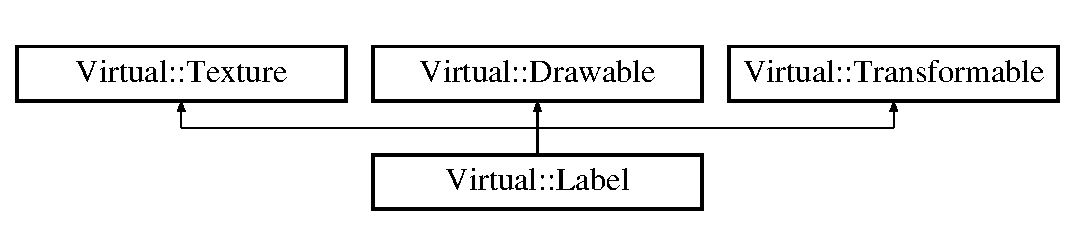
\includegraphics[height=3.000000cm]{class_virtual_1_1_label}
\end{center}
\end{figure}
\subsection*{Public Member Functions}
\begin{DoxyCompactItemize}
\item 
void \hyperlink{class_virtual_1_1_label_a077d7852f09f940a9932f63fb616351c}{draw} (S\+D\+L\+\_\+\+Renderer $\ast$, \hyperlink{class_virtual_1_1_camera}{Camera} \&)
\begin{DoxyCompactList}\small\item\em Function that use engine to draw object. \end{DoxyCompactList}\item 
void \hyperlink{class_virtual_1_1_label_adf4f738abab5dca3815a9c6f4124eec6}{set\+Color} (\hyperlink{struct_virtual_1_1_color}{Color} color)
\begin{DoxyCompactList}\small\item\em Setting font color. \end{DoxyCompactList}\item 
void \hyperlink{class_virtual_1_1_label_a643dca9416c60c78b1b1fc234ed6964c}{set\+Font} (std\+::shared\+\_\+ptr$<$ \hyperlink{class_virtual_1_1_font}{Font} $>$ font)
\begin{DoxyCompactList}\small\item\em Setting \hyperlink{class_virtual_1_1_font}{Font} into \hyperlink{class_virtual_1_1_label}{Label}. \end{DoxyCompactList}\item 
void \hyperlink{class_virtual_1_1_label_a20e22a03b54b9851ad675c491df1ae75}{set\+Size} (int size)
\begin{DoxyCompactList}\small\item\em Setting \hyperlink{class_virtual_1_1_font}{Font} size. \end{DoxyCompactList}\item 
void \hyperlink{class_virtual_1_1_label_a1b737a96ea06f214120c61dc2465536f}{set\+Text} (std\+::string text)
\end{DoxyCompactItemize}
\subsection*{Additional Inherited Members}


\subsection{Detailed Description}
Simple sprite dynamic class, like \hyperlink{class_virtual_1_1_sprite}{Sprite}. 

\subsection{Member Function Documentation}
\hypertarget{class_virtual_1_1_label_a077d7852f09f940a9932f63fb616351c}{}\label{class_virtual_1_1_label_a077d7852f09f940a9932f63fb616351c} 
\index{Virtual\+::\+Label@{Virtual\+::\+Label}!draw@{draw}}
\index{draw@{draw}!Virtual\+::\+Label@{Virtual\+::\+Label}}
\subsubsection{\texorpdfstring{draw()}{draw()}}
{\footnotesize\ttfamily void Virtual\+::\+Label\+::draw (\begin{DoxyParamCaption}\item[{S\+D\+L\+\_\+\+Renderer $\ast$}]{,  }\item[{\hyperlink{class_virtual_1_1_camera}{Camera} \&}]{ }\end{DoxyParamCaption})\hspace{0.3cm}{\ttfamily [virtual]}}



Function that use engine to draw object. 


\begin{DoxyParams}{Parameters}
{\em renderer} & -\/ pointer into S\+D\+L\+\_\+\+Renderer \\
\hline
{\em camera} & -\/ reference to camera in engine \\
\hline
\end{DoxyParams}


Reimplemented from \hyperlink{class_virtual_1_1_sprite_a57f581e0307ab2b2dd7c6922dba2a057}{Virtual\+::\+Sprite}.

\hypertarget{class_virtual_1_1_label_adf4f738abab5dca3815a9c6f4124eec6}{}\label{class_virtual_1_1_label_adf4f738abab5dca3815a9c6f4124eec6} 
\index{Virtual\+::\+Label@{Virtual\+::\+Label}!set\+Color@{set\+Color}}
\index{set\+Color@{set\+Color}!Virtual\+::\+Label@{Virtual\+::\+Label}}
\subsubsection{\texorpdfstring{set\+Color()}{setColor()}}
{\footnotesize\ttfamily void Virtual\+::\+Label\+::set\+Color (\begin{DoxyParamCaption}\item[{\hyperlink{struct_virtual_1_1_color}{Color}}]{color }\end{DoxyParamCaption})}



Setting font color. 


\begin{DoxyParams}{Parameters}
{\em color} & -\/ R\+GB \hyperlink{struct_virtual_1_1_color}{Color} structure \\
\hline
\end{DoxyParams}
\hypertarget{class_virtual_1_1_label_a643dca9416c60c78b1b1fc234ed6964c}{}\label{class_virtual_1_1_label_a643dca9416c60c78b1b1fc234ed6964c} 
\index{Virtual\+::\+Label@{Virtual\+::\+Label}!set\+Font@{set\+Font}}
\index{set\+Font@{set\+Font}!Virtual\+::\+Label@{Virtual\+::\+Label}}
\subsubsection{\texorpdfstring{set\+Font()}{setFont()}}
{\footnotesize\ttfamily void Virtual\+::\+Label\+::set\+Font (\begin{DoxyParamCaption}\item[{std\+::shared\+\_\+ptr$<$ \hyperlink{class_virtual_1_1_font}{Font} $>$}]{font }\end{DoxyParamCaption})}



Setting \hyperlink{class_virtual_1_1_font}{Font} into \hyperlink{class_virtual_1_1_label}{Label}. 


\begin{DoxyParams}{Parameters}
{\em font} & -\/ Dynamic pointer into \hyperlink{class_virtual_1_1_font}{Font} \\
\hline
\end{DoxyParams}
\hypertarget{class_virtual_1_1_label_a20e22a03b54b9851ad675c491df1ae75}{}\label{class_virtual_1_1_label_a20e22a03b54b9851ad675c491df1ae75} 
\index{Virtual\+::\+Label@{Virtual\+::\+Label}!set\+Size@{set\+Size}}
\index{set\+Size@{set\+Size}!Virtual\+::\+Label@{Virtual\+::\+Label}}
\subsubsection{\texorpdfstring{set\+Size()}{setSize()}}
{\footnotesize\ttfamily void Virtual\+::\+Label\+::set\+Size (\begin{DoxyParamCaption}\item[{int}]{size }\end{DoxyParamCaption})}



Setting \hyperlink{class_virtual_1_1_font}{Font} size. 


\begin{DoxyParams}{Parameters}
{\em size} & -\/ integer number \\
\hline
\end{DoxyParams}
\hypertarget{class_virtual_1_1_label_a1b737a96ea06f214120c61dc2465536f}{}\label{class_virtual_1_1_label_a1b737a96ea06f214120c61dc2465536f} 
\index{Virtual\+::\+Label@{Virtual\+::\+Label}!set\+Text@{set\+Text}}
\index{set\+Text@{set\+Text}!Virtual\+::\+Label@{Virtual\+::\+Label}}
\subsubsection{\texorpdfstring{set\+Text()}{setText()}}
{\footnotesize\ttfamily void Virtual\+::\+Label\+::set\+Text (\begin{DoxyParamCaption}\item[{std\+::string}]{text }\end{DoxyParamCaption})}


\begin{DoxyParams}{Parameters}
{\em text} & -\/ string to drawing \\
\hline
\end{DoxyParams}


The documentation for this class was generated from the following file\+:\begin{DoxyCompactItemize}
\item 
include/\+Virtual\+Eye/Render\+Utils.\+hpp\end{DoxyCompactItemize}

\hypertarget{struct_virtual_1_1_map}{}\section{Virtual\+:\+:Map Struct Reference}
\label{struct_virtual_1_1_map}\index{Virtual\+::\+Map@{Virtual\+::\+Map}}


Info about map.  




{\ttfamily \#include $<$Map.\+hpp$>$}

\subsection*{Public Member Functions}
\begin{DoxyCompactItemize}
\item 
std\+::shared\+\_\+ptr$<$ \hyperlink{class_virtual_1_1_tile}{Tile} $>$ \hyperlink{struct_virtual_1_1_map_ae92e86e0da301c4481718bc871086013}{get\+Tile\+At} (\hyperlink{struct_virtual_1_1_vector2}{Vector2}$<$ int $>$ position)
\begin{DoxyCompactList}\small\item\em Numbers type of one single tile. \end{DoxyCompactList}\end{DoxyCompactItemize}
\subsection*{Public Attributes}
\begin{DoxyCompactItemize}
\item 
\hypertarget{struct_virtual_1_1_map_a80eba30b23a223e38892fb54ac3fd5ae}{}\label{struct_virtual_1_1_map_a80eba30b23a223e38892fb54ac3fd5ae} 
std\+::vector$<$ std\+::vector$<$ int $>$ $>$ \hyperlink{struct_virtual_1_1_map_a80eba30b23a223e38892fb54ac3fd5ae}{numbers}
\begin{DoxyCompactList}\small\item\em Numbers type of one single tile. \end{DoxyCompactList}\item 
\hypertarget{struct_virtual_1_1_map_a008dc98ea15efda9eebdafdde794b26c}{}\label{struct_virtual_1_1_map_a008dc98ea15efda9eebdafdde794b26c} 
std\+::vector$<$ std\+::vector$<$ std\+::shared\+\_\+ptr$<$ \hyperlink{class_virtual_1_1_tile}{Tile} $>$ $>$ $>$ \hyperlink{struct_virtual_1_1_map_a008dc98ea15efda9eebdafdde794b26c}{tiles}
\begin{DoxyCompactList}\small\item\em Storage of all tiles of map. \end{DoxyCompactList}\item 
\hypertarget{struct_virtual_1_1_map_ab20e5047996b454cbbc815be37ac9c6c}{}\label{struct_virtual_1_1_map_ab20e5047996b454cbbc815be37ac9c6c} 
\hyperlink{class_virtual_1_1_texture}{Texture} \hyperlink{struct_virtual_1_1_map_ab20e5047996b454cbbc815be37ac9c6c}{texture}
\begin{DoxyCompactList}\small\item\em Tileset texture. \end{DoxyCompactList}\item 
\hypertarget{struct_virtual_1_1_map_aa03b68bb0d0944fd7ce08cff9e1ff9f6}{}\label{struct_virtual_1_1_map_aa03b68bb0d0944fd7ce08cff9e1ff9f6} 
std\+::string \hyperlink{struct_virtual_1_1_map_aa03b68bb0d0944fd7ce08cff9e1ff9f6}{map\+Path}
\begin{DoxyCompactList}\small\item\em Path to map definition ($\ast$.iom) \end{DoxyCompactList}\item 
\hypertarget{struct_virtual_1_1_map_a89d67a1e3ae34917ed85a4d73e297987}{}\label{struct_virtual_1_1_map_a89d67a1e3ae34917ed85a4d73e297987} 
std\+::string \hyperlink{struct_virtual_1_1_map_a89d67a1e3ae34917ed85a4d73e297987}{texture\+Path}
\begin{DoxyCompactList}\small\item\em Path to tilset. \end{DoxyCompactList}\item 
\hypertarget{struct_virtual_1_1_map_a9441a7d20d769a4237be8d657e66508b}{}\label{struct_virtual_1_1_map_a9441a7d20d769a4237be8d657e66508b} 
int \hyperlink{struct_virtual_1_1_map_a9441a7d20d769a4237be8d657e66508b}{tiles\+Size}
\begin{DoxyCompactList}\small\item\em Width and height of one tile. \end{DoxyCompactList}\item 
\hypertarget{struct_virtual_1_1_map_a721b68e91377a8e5e29596ad633b61e6}{}\label{struct_virtual_1_1_map_a721b68e91377a8e5e29596ad633b61e6} 
int \hyperlink{struct_virtual_1_1_map_a721b68e91377a8e5e29596ad633b61e6}{max\+Number}
\begin{DoxyCompactList}\small\item\em The biggest number of tile type. \end{DoxyCompactList}\item 
\hypertarget{struct_virtual_1_1_map_ad0b8913dd7e67b7d0d73fe7f2b9c0ab8}{}\label{struct_virtual_1_1_map_ad0b8913dd7e67b7d0d73fe7f2b9c0ab8} 
int \hyperlink{struct_virtual_1_1_map_ad0b8913dd7e67b7d0d73fe7f2b9c0ab8}{width}
\begin{DoxyCompactList}\small\item\em Width of map in pixel. \end{DoxyCompactList}\item 
\hypertarget{struct_virtual_1_1_map_ad0b22c3d2f1be10c717085dac12f8dcb}{}\label{struct_virtual_1_1_map_ad0b22c3d2f1be10c717085dac12f8dcb} 
int \hyperlink{struct_virtual_1_1_map_ad0b22c3d2f1be10c717085dac12f8dcb}{height}
\begin{DoxyCompactList}\small\item\em Height of map in pixel. \end{DoxyCompactList}\end{DoxyCompactItemize}


\subsection{Detailed Description}
Info about map. 

\subsection{Member Function Documentation}
\hypertarget{struct_virtual_1_1_map_ae92e86e0da301c4481718bc871086013}{}\label{struct_virtual_1_1_map_ae92e86e0da301c4481718bc871086013} 
\index{Virtual\+::\+Map@{Virtual\+::\+Map}!get\+Tile\+At@{get\+Tile\+At}}
\index{get\+Tile\+At@{get\+Tile\+At}!Virtual\+::\+Map@{Virtual\+::\+Map}}
\subsubsection{\texorpdfstring{get\+Tile\+At()}{getTileAt()}}
{\footnotesize\ttfamily std\+::shared\+\_\+ptr$<$\hyperlink{class_virtual_1_1_tile}{Tile}$>$ Virtual\+::\+Map\+::get\+Tile\+At (\begin{DoxyParamCaption}\item[{\hyperlink{struct_virtual_1_1_vector2}{Vector2}$<$ int $>$}]{position }\end{DoxyParamCaption})\hspace{0.3cm}{\ttfamily [inline]}}



Numbers type of one single tile. 


\begin{DoxyParams}{Parameters}
{\em position} & -\/ position of sprite in the table (like \hyperlink{struct_virtual_1_1_vector2}{Vector2$<$int$>$(2, 2)} to get the tile at 2\+:2 coords)\\
\hline
\end{DoxyParams}
\begin{DoxyReturn}{Returns}
Reference to tile by they position in table 
\end{DoxyReturn}


The documentation for this struct was generated from the following file\+:\begin{DoxyCompactItemize}
\item 
include/\+Virtual\+Eye/Map.\+hpp\end{DoxyCompactItemize}

\hypertarget{class_virtual_1_1_music}{}\section{Virtual\+:\+:Music Class Reference}
\label{class_virtual_1_1_music}\index{Virtual\+::\+Music@{Virtual\+::\+Music}}
Inheritance diagram for Virtual\+:\+:Music\+:\begin{figure}[H]
\begin{center}
\leavevmode
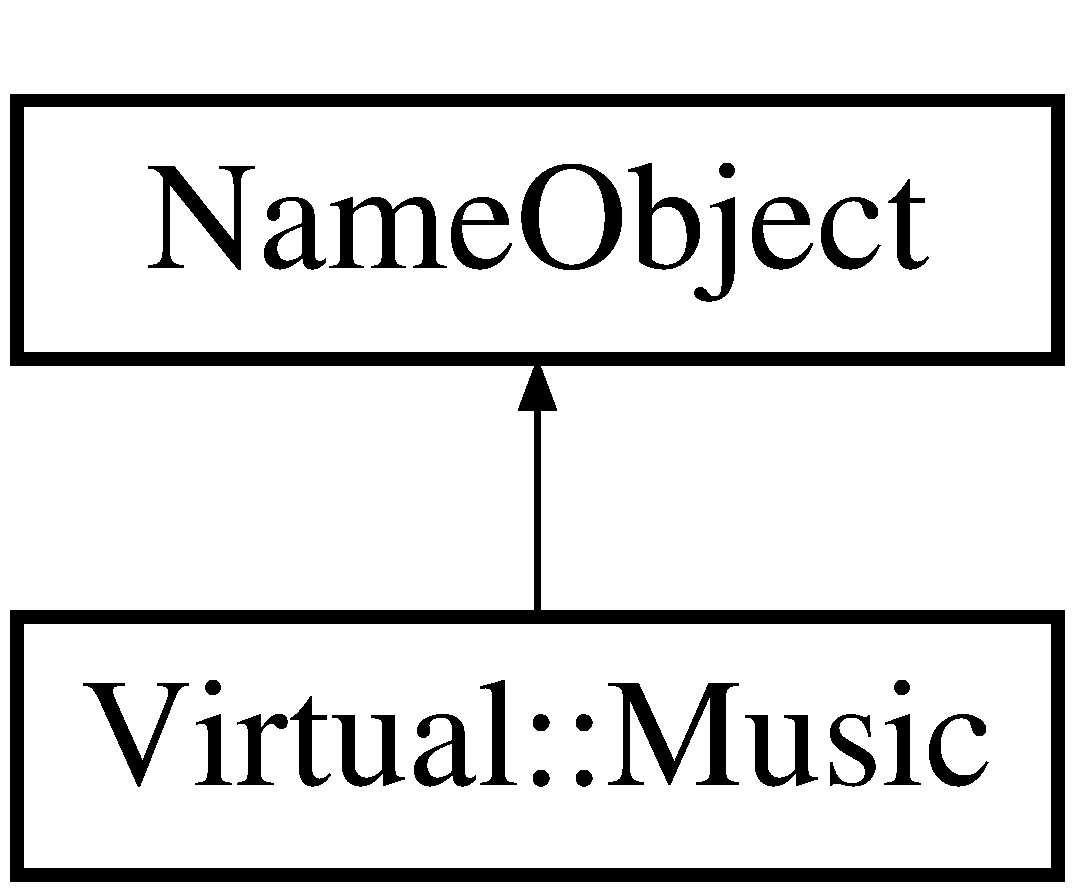
\includegraphics[height=2.000000cm]{class_virtual_1_1_music}
\end{center}
\end{figure}
\subsection*{Public Member Functions}
\begin{DoxyCompactItemize}
\item 
\hypertarget{class_virtual_1_1_music_a0fc4f3eab54d97628eb130a00794ecd8}{}\label{class_virtual_1_1_music_a0fc4f3eab54d97628eb130a00794ecd8} 
void {\bfseries load\+Music} (Mix\+\_\+\+Music $\ast$music)
\item 
\hypertarget{class_virtual_1_1_music_a24b6650bc34f9a2ad0f38d8ecf0092d5}{}\label{class_virtual_1_1_music_a24b6650bc34f9a2ad0f38d8ecf0092d5} 
void {\bfseries play} ()
\end{DoxyCompactItemize}


The documentation for this class was generated from the following file\+:\begin{DoxyCompactItemize}
\item 
include/\+Virtual\+Eye/Dynamic\+Pointers.\+hpp\end{DoxyCompactItemize}

\hypertarget{class_virtual_1_1_music_player}{}\section{Virtual\+:\+:Music\+Player Class Reference}
\label{class_virtual_1_1_music_player}\index{Virtual\+::\+Music\+Player@{Virtual\+::\+Music\+Player}}


Class to play music.  




{\ttfamily \#include $<$Music\+Player.\+hpp$>$}

\subsection*{Public Member Functions}
\begin{DoxyCompactItemize}
\item 
\hypertarget{class_virtual_1_1_music_player_a3d13da4502c0dd17f1f5660e9f994620}{}\label{class_virtual_1_1_music_player_a3d13da4502c0dd17f1f5660e9f994620} 
void {\bfseries load\+Music} (std\+::string path, std\+::string name)
\item 
\hypertarget{class_virtual_1_1_music_player_ac7181d557661bd77daac91aa62f565f6}{}\label{class_virtual_1_1_music_player_ac7181d557661bd77daac91aa62f565f6} 
void {\bfseries play\+Music} (std\+::string name)
\end{DoxyCompactItemize}


\subsection{Detailed Description}
Class to play music. 

The documentation for this class was generated from the following file\+:\begin{DoxyCompactItemize}
\item 
include/\+Virtual\+Eye/Music\+Player.\+hpp\end{DoxyCompactItemize}

\hypertarget{class_name_object}{}\section{Name\+Object Class Reference}
\label{class_name_object}\index{Name\+Object@{Name\+Object}}
Inheritance diagram for Name\+Object\+:\begin{figure}[H]
\begin{center}
\leavevmode
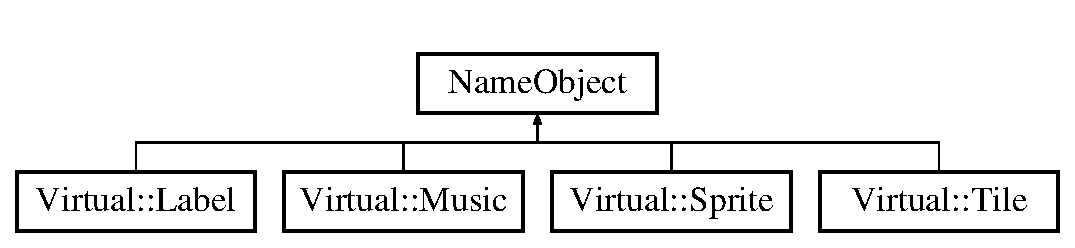
\includegraphics[height=2.000000cm]{class_name_object}
\end{center}
\end{figure}
\subsection*{Public Member Functions}
\begin{DoxyCompactItemize}
\item 
void \hyperlink{class_name_object_a4172d35244e556278ae8b7dae238c16a}{set\+Name} (std\+::string name)
\begin{DoxyCompactList}\small\item\em Sets name of object. \end{DoxyCompactList}\item 
std\+::string \hyperlink{class_name_object_a8504c3c36a4d3983116866153e60bd7d}{get\+Name} (void)
\end{DoxyCompactItemize}


\subsection{Member Function Documentation}
\hypertarget{class_name_object_a8504c3c36a4d3983116866153e60bd7d}{}\label{class_name_object_a8504c3c36a4d3983116866153e60bd7d} 
\index{Name\+Object@{Name\+Object}!get\+Name@{get\+Name}}
\index{get\+Name@{get\+Name}!Name\+Object@{Name\+Object}}
\subsubsection{\texorpdfstring{get\+Name()}{getName()}}
{\footnotesize\ttfamily std\+::string Name\+Object\+::get\+Name (\begin{DoxyParamCaption}\item[{void}]{ }\end{DoxyParamCaption})\hspace{0.3cm}{\ttfamily [inline]}}

\begin{DoxyReturn}{Returns}
name of object 
\end{DoxyReturn}
\hypertarget{class_name_object_a4172d35244e556278ae8b7dae238c16a}{}\label{class_name_object_a4172d35244e556278ae8b7dae238c16a} 
\index{Name\+Object@{Name\+Object}!set\+Name@{set\+Name}}
\index{set\+Name@{set\+Name}!Name\+Object@{Name\+Object}}
\subsubsection{\texorpdfstring{set\+Name()}{setName()}}
{\footnotesize\ttfamily void Name\+Object\+::set\+Name (\begin{DoxyParamCaption}\item[{std\+::string}]{name }\end{DoxyParamCaption})\hspace{0.3cm}{\ttfamily [inline]}}



Sets name of object. 


\begin{DoxyParams}{Parameters}
{\em name} & -\/ name of object \\
\hline
\end{DoxyParams}


The documentation for this class was generated from the following file\+:\begin{DoxyCompactItemize}
\item 
include/\+Virtual\+Eye/Name\+Object.\+hpp\end{DoxyCompactItemize}

\hypertarget{struct_virtual_1_1_rectangle}{}\section{Virtual\+:\+:Rectangle$<$ T $>$ Struct Template Reference}
\label{struct_virtual_1_1_rectangle}\index{Virtual\+::\+Rectangle$<$ T $>$@{Virtual\+::\+Rectangle$<$ T $>$}}


The simple coorinates of \hyperlink{struct_virtual_1_1_rectangle}{Rectangle}.  




{\ttfamily \#include $<$Math.\+hpp$>$}

\subsection*{Public Member Functions}
\begin{DoxyCompactItemize}
\item 
\hyperlink{struct_virtual_1_1_rectangle_ae2d69ec79c6caf39973a5226995d5437}{Rectangle} ()
\begin{DoxyCompactList}\small\item\em Default zero constructor. \end{DoxyCompactList}\item 
\hyperlink{struct_virtual_1_1_rectangle_a7cb26cfb2eee27a70fa1e7cae997c72c}{Rectangle} (T xx, T yy, T ww, T hh)
\begin{DoxyCompactList}\small\item\em Default custom constructor. \end{DoxyCompactList}\item 
void \hyperlink{struct_virtual_1_1_rectangle_abe71777391c0d70a523bde7be00054df}{set\+Position} (T xx, T yy)
\begin{DoxyCompactList}\small\item\em Setting position of x and y of upper-\/left angle. \end{DoxyCompactList}\item 
void \hyperlink{struct_virtual_1_1_rectangle_a7894397b7dc0a3ef61b5dfd26e40dcfa}{set\+Parametres} (T ww, T hh)
\begin{DoxyCompactList}\small\item\em Setting width and height of \hyperlink{struct_virtual_1_1_rectangle}{Rectangle}. \end{DoxyCompactList}\end{DoxyCompactItemize}
\subsection*{Public Attributes}
\begin{DoxyCompactItemize}
\item 
\hypertarget{struct_virtual_1_1_rectangle_a767eced304189f1f9fc9a0c8b329a679}{}\label{struct_virtual_1_1_rectangle_a767eced304189f1f9fc9a0c8b329a679} 
T {\bfseries x}
\item 
\hypertarget{struct_virtual_1_1_rectangle_a0f392a2d77d2b91b2e65e4badd3f37aa}{}\label{struct_virtual_1_1_rectangle_a0f392a2d77d2b91b2e65e4badd3f37aa} 
T {\bfseries y}
\item 
\hypertarget{struct_virtual_1_1_rectangle_af60772870e4e51ffbce47f827d70e405}{}\label{struct_virtual_1_1_rectangle_af60772870e4e51ffbce47f827d70e405} 
T {\bfseries w}
\item 
\hypertarget{struct_virtual_1_1_rectangle_a3b60edf80bba3f7f48f0c57ad44b34ed}{}\label{struct_virtual_1_1_rectangle_a3b60edf80bba3f7f48f0c57ad44b34ed} 
T {\bfseries h}
\end{DoxyCompactItemize}


\subsection{Detailed Description}
\subsubsection*{template$<$typename T$>$\newline
struct Virtual\+::\+Rectangle$<$ T $>$}

The simple coorinates of \hyperlink{struct_virtual_1_1_rectangle}{Rectangle}. 

\hyperlink{struct_virtual_1_1_rectangle}{Rectangle} class manage the parametres of the \hyperlink{struct_virtual_1_1_rectangle}{Rectangle} like width, height of they etc. 

\subsection{Constructor \& Destructor Documentation}
\hypertarget{struct_virtual_1_1_rectangle_ae2d69ec79c6caf39973a5226995d5437}{}\label{struct_virtual_1_1_rectangle_ae2d69ec79c6caf39973a5226995d5437} 
\index{Virtual\+::\+Rectangle@{Virtual\+::\+Rectangle}!Rectangle@{Rectangle}}
\index{Rectangle@{Rectangle}!Virtual\+::\+Rectangle@{Virtual\+::\+Rectangle}}
\subsubsection{\texorpdfstring{Rectangle()}{Rectangle()}\hspace{0.1cm}{\footnotesize\ttfamily [1/2]}}
{\footnotesize\ttfamily template$<$typename T$>$ \\
\hyperlink{struct_virtual_1_1_rectangle}{Virtual\+::\+Rectangle}$<$ T $>$\+::\hyperlink{struct_virtual_1_1_rectangle}{Rectangle} (\begin{DoxyParamCaption}{ }\end{DoxyParamCaption})\hspace{0.3cm}{\ttfamily [inline]}}



Default zero constructor. 

This constructor append of each variables zero. \hypertarget{struct_virtual_1_1_rectangle_a7cb26cfb2eee27a70fa1e7cae997c72c}{}\label{struct_virtual_1_1_rectangle_a7cb26cfb2eee27a70fa1e7cae997c72c} 
\index{Virtual\+::\+Rectangle@{Virtual\+::\+Rectangle}!Rectangle@{Rectangle}}
\index{Rectangle@{Rectangle}!Virtual\+::\+Rectangle@{Virtual\+::\+Rectangle}}
\subsubsection{\texorpdfstring{Rectangle()}{Rectangle()}\hspace{0.1cm}{\footnotesize\ttfamily [2/2]}}
{\footnotesize\ttfamily template$<$typename T$>$ \\
\hyperlink{struct_virtual_1_1_rectangle}{Virtual\+::\+Rectangle}$<$ T $>$\+::\hyperlink{struct_virtual_1_1_rectangle}{Rectangle} (\begin{DoxyParamCaption}\item[{T}]{xx,  }\item[{T}]{yy,  }\item[{T}]{ww,  }\item[{T}]{hh }\end{DoxyParamCaption})\hspace{0.3cm}{\ttfamily [inline]}}



Default custom constructor. 


\begin{DoxyParams}{Parameters}
{\em xx} & -\/ x value \\
\hline
{\em yy} & -\/ y value \\
\hline
{\em ww} & -\/ w value \\
\hline
{\em hh} & -\/ h value\\
\hline
\end{DoxyParams}
This constructor append of each variables given values. 

\subsection{Member Function Documentation}
\hypertarget{struct_virtual_1_1_rectangle_a7894397b7dc0a3ef61b5dfd26e40dcfa}{}\label{struct_virtual_1_1_rectangle_a7894397b7dc0a3ef61b5dfd26e40dcfa} 
\index{Virtual\+::\+Rectangle@{Virtual\+::\+Rectangle}!set\+Parametres@{set\+Parametres}}
\index{set\+Parametres@{set\+Parametres}!Virtual\+::\+Rectangle@{Virtual\+::\+Rectangle}}
\subsubsection{\texorpdfstring{set\+Parametres()}{setParametres()}}
{\footnotesize\ttfamily template$<$typename T$>$ \\
void \hyperlink{struct_virtual_1_1_rectangle}{Virtual\+::\+Rectangle}$<$ T $>$\+::set\+Parametres (\begin{DoxyParamCaption}\item[{T}]{ww,  }\item[{T}]{hh }\end{DoxyParamCaption})\hspace{0.3cm}{\ttfamily [inline]}}



Setting width and height of \hyperlink{struct_virtual_1_1_rectangle}{Rectangle}. 


\begin{DoxyParams}{Parameters}
{\em ww} & -\/ w value \\
\hline
{\em hh} & -\/ h value \\
\hline
\end{DoxyParams}
\hypertarget{struct_virtual_1_1_rectangle_abe71777391c0d70a523bde7be00054df}{}\label{struct_virtual_1_1_rectangle_abe71777391c0d70a523bde7be00054df} 
\index{Virtual\+::\+Rectangle@{Virtual\+::\+Rectangle}!set\+Position@{set\+Position}}
\index{set\+Position@{set\+Position}!Virtual\+::\+Rectangle@{Virtual\+::\+Rectangle}}
\subsubsection{\texorpdfstring{set\+Position()}{setPosition()}}
{\footnotesize\ttfamily template$<$typename T$>$ \\
void \hyperlink{struct_virtual_1_1_rectangle}{Virtual\+::\+Rectangle}$<$ T $>$\+::set\+Position (\begin{DoxyParamCaption}\item[{T}]{xx,  }\item[{T}]{yy }\end{DoxyParamCaption})\hspace{0.3cm}{\ttfamily [inline]}}



Setting position of x and y of upper-\/left angle. 


\begin{DoxyParams}{Parameters}
{\em xx} & -\/ x value \\
\hline
{\em yy} & -\/ y value \\
\hline
\end{DoxyParams}


The documentation for this struct was generated from the following file\+:\begin{DoxyCompactItemize}
\item 
include/\+Virtual\+Eye/Math.\+hpp\end{DoxyCompactItemize}

\hypertarget{class_virtual_1_1_renderer}{}\section{Virtual\+:\+:Renderer Class Reference}
\label{class_virtual_1_1_renderer}\index{Virtual\+::\+Renderer@{Virtual\+::\+Renderer}}


Management of current scene.  




{\ttfamily \#include $<$Renderer.\+hpp$>$}

\subsection*{Public Member Functions}
\begin{DoxyCompactItemize}
\item 
\hypertarget{class_virtual_1_1_renderer_a2474ee636beae9079b5283c4c5729acc}{}\label{class_virtual_1_1_renderer_a2474ee636beae9079b5283c4c5729acc} 
{\bfseries Renderer} (S\+D\+L\+\_\+\+Window $\ast$)
\item 
void \hyperlink{class_virtual_1_1_renderer_ae1151907121db309b9d1b650b3dbe076}{draw} (\hyperlink{class_virtual_1_1_camera}{Camera} \&camera)
\begin{DoxyCompactList}\small\item\em Draws the scene. \end{DoxyCompactList}\item 
void \hyperlink{class_virtual_1_1_renderer_a2c4ba07e2388d77606f77cf10e5af0d1}{clear\+Scene} (void)
\begin{DoxyCompactList}\small\item\em Clearing the scene. \end{DoxyCompactList}\item 
void \hyperlink{class_virtual_1_1_renderer_a55910b43e187352052f2b51019fd16ef}{load\+Sprite} (std\+::string path, \hyperlink{struct_virtual_1_1_vector2}{Vector2}$<$ int $>$ position, std\+::string name, bool is\+Displaying=false)
\begin{DoxyCompactList}\small\item\em Loading sprite. \end{DoxyCompactList}\item 
void \hyperlink{class_virtual_1_1_renderer_a6addf8a58c9024701a5da4fe814561e8}{load\+Label} (std\+::string path, std\+::string text, \hyperlink{struct_virtual_1_1_vector2}{Vector2}$<$ int $>$ position, std\+::string name, \hyperlink{struct_virtual_1_1_color}{Color} color, int size=30, bool is\+Displaying=false)
\begin{DoxyCompactList}\small\item\em Loading sprite. \end{DoxyCompactList}\item 
\hyperlink{struct_virtual_1_1_vector2}{Vector2}$<$ int $>$ \hyperlink{class_virtual_1_1_renderer_a8b1576675d456d42a8b08bfb6a2d50af}{load\+Map} (std\+::string path)
\begin{DoxyCompactList}\small\item\em Loads map. \end{DoxyCompactList}\item 
std\+::shared\+\_\+ptr$<$ \hyperlink{struct_virtual_1_1_map}{Map} $>$ \hyperlink{class_virtual_1_1_renderer_aaa8e493c4e05d5eaca42604555d3b419}{get\+Map} (void)
\item 
\hyperlink{class_virtual_1_1_sprite}{Sprite} \& \hyperlink{class_virtual_1_1_renderer_ae2be5bddf056acb2c00f77fb6f0afa6c}{get\+Sprite\+By\+Id} (std\+::string name)
\item 
\hyperlink{class_virtual_1_1_label}{Label} \& \hyperlink{class_virtual_1_1_renderer_a11f3dbe70c634fb465b5b21d43618f5d}{get\+Label\+By\+Id} (std\+::string name)
\end{DoxyCompactItemize}


\subsection{Detailed Description}
Management of current scene. 

Class of renderer manage the scene by loading sprite, label to they, cleaning the scene etc. 

\subsection{Member Function Documentation}
\hypertarget{class_virtual_1_1_renderer_a2c4ba07e2388d77606f77cf10e5af0d1}{}\label{class_virtual_1_1_renderer_a2c4ba07e2388d77606f77cf10e5af0d1} 
\index{Virtual\+::\+Renderer@{Virtual\+::\+Renderer}!clear\+Scene@{clear\+Scene}}
\index{clear\+Scene@{clear\+Scene}!Virtual\+::\+Renderer@{Virtual\+::\+Renderer}}
\subsubsection{\texorpdfstring{clear\+Scene()}{clearScene()}}
{\footnotesize\ttfamily void Virtual\+::\+Renderer\+::clear\+Scene (\begin{DoxyParamCaption}\item[{void}]{ }\end{DoxyParamCaption})}



Clearing the scene. 

Deleting all vector and cleaning them. Nothing will not rendering after that. \hypertarget{class_virtual_1_1_renderer_ae1151907121db309b9d1b650b3dbe076}{}\label{class_virtual_1_1_renderer_ae1151907121db309b9d1b650b3dbe076} 
\index{Virtual\+::\+Renderer@{Virtual\+::\+Renderer}!draw@{draw}}
\index{draw@{draw}!Virtual\+::\+Renderer@{Virtual\+::\+Renderer}}
\subsubsection{\texorpdfstring{draw()}{draw()}}
{\footnotesize\ttfamily void Virtual\+::\+Renderer\+::draw (\begin{DoxyParamCaption}\item[{\hyperlink{class_virtual_1_1_camera}{Camera} \&}]{camera }\end{DoxyParamCaption})}



Draws the scene. 


\begin{DoxyParams}{Parameters}
{\em camera} & the reference to camera object\\
\hline
\end{DoxyParams}
Draws the scene on the screen. \hypertarget{class_virtual_1_1_renderer_a11f3dbe70c634fb465b5b21d43618f5d}{}\label{class_virtual_1_1_renderer_a11f3dbe70c634fb465b5b21d43618f5d} 
\index{Virtual\+::\+Renderer@{Virtual\+::\+Renderer}!get\+Label\+By\+Id@{get\+Label\+By\+Id}}
\index{get\+Label\+By\+Id@{get\+Label\+By\+Id}!Virtual\+::\+Renderer@{Virtual\+::\+Renderer}}
\subsubsection{\texorpdfstring{get\+Label\+By\+Id()}{getLabelById()}}
{\footnotesize\ttfamily \hyperlink{class_virtual_1_1_label}{Label}\& Virtual\+::\+Renderer\+::get\+Label\+By\+Id (\begin{DoxyParamCaption}\item[{std\+::string}]{name }\end{DoxyParamCaption})}

\begin{DoxyReturn}{Returns}
The object of label by the name
\end{DoxyReturn}

\begin{DoxyParams}{Parameters}
{\em name} & -\/ name of searched label \\
\hline
\end{DoxyParams}
\hypertarget{class_virtual_1_1_renderer_aaa8e493c4e05d5eaca42604555d3b419}{}\label{class_virtual_1_1_renderer_aaa8e493c4e05d5eaca42604555d3b419} 
\index{Virtual\+::\+Renderer@{Virtual\+::\+Renderer}!get\+Map@{get\+Map}}
\index{get\+Map@{get\+Map}!Virtual\+::\+Renderer@{Virtual\+::\+Renderer}}
\subsubsection{\texorpdfstring{get\+Map()}{getMap()}}
{\footnotesize\ttfamily std\+::shared\+\_\+ptr$<$\hyperlink{struct_virtual_1_1_map}{Map}$>$ Virtual\+::\+Renderer\+::get\+Map (\begin{DoxyParamCaption}\item[{void}]{ }\end{DoxyParamCaption})}

\begin{DoxyReturn}{Returns}
Dynamic pointer into map info
\end{DoxyReturn}
Returning map info like width and height, number of tiles etc. \hypertarget{class_virtual_1_1_renderer_ae2be5bddf056acb2c00f77fb6f0afa6c}{}\label{class_virtual_1_1_renderer_ae2be5bddf056acb2c00f77fb6f0afa6c} 
\index{Virtual\+::\+Renderer@{Virtual\+::\+Renderer}!get\+Sprite\+By\+Id@{get\+Sprite\+By\+Id}}
\index{get\+Sprite\+By\+Id@{get\+Sprite\+By\+Id}!Virtual\+::\+Renderer@{Virtual\+::\+Renderer}}
\subsubsection{\texorpdfstring{get\+Sprite\+By\+Id()}{getSpriteById()}}
{\footnotesize\ttfamily \hyperlink{class_virtual_1_1_sprite}{Sprite}\& Virtual\+::\+Renderer\+::get\+Sprite\+By\+Id (\begin{DoxyParamCaption}\item[{std\+::string}]{name }\end{DoxyParamCaption})}

\begin{DoxyReturn}{Returns}
The object of sprite by the name
\end{DoxyReturn}

\begin{DoxyParams}{Parameters}
{\em name} & -\/ name of searched sprite \\
\hline
\end{DoxyParams}
\hypertarget{class_virtual_1_1_renderer_a6addf8a58c9024701a5da4fe814561e8}{}\label{class_virtual_1_1_renderer_a6addf8a58c9024701a5da4fe814561e8} 
\index{Virtual\+::\+Renderer@{Virtual\+::\+Renderer}!load\+Label@{load\+Label}}
\index{load\+Label@{load\+Label}!Virtual\+::\+Renderer@{Virtual\+::\+Renderer}}
\subsubsection{\texorpdfstring{load\+Label()}{loadLabel()}}
{\footnotesize\ttfamily void Virtual\+::\+Renderer\+::load\+Label (\begin{DoxyParamCaption}\item[{std\+::string}]{path,  }\item[{std\+::string}]{text,  }\item[{\hyperlink{struct_virtual_1_1_vector2}{Vector2}$<$ int $>$}]{position,  }\item[{std\+::string}]{name,  }\item[{\hyperlink{struct_virtual_1_1_color}{Color}}]{color,  }\item[{int}]{size = {\ttfamily 30},  }\item[{bool}]{is\+Displaying = {\ttfamily false} }\end{DoxyParamCaption})}



Loading sprite. 


\begin{DoxyParams}{Parameters}
{\em path} & -\/ path to font \\
\hline
{\em text} & -\/ text on label \\
\hline
{\em position} & -\/ integer vector of the position relative to window \\
\hline
{\em name} & -\/ identity name of sprite \\
\hline
{\em color} & -\/ color of text in label \\
\hline
{\em size} & -\/ size of font \\
\hline
{\em is\+Displaying} & -\/ fact is the object was displaying\\
\hline
\end{DoxyParams}
Creating label, setting position and name of they and pushing the instance into label vector. \hypertarget{class_virtual_1_1_renderer_a8b1576675d456d42a8b08bfb6a2d50af}{}\label{class_virtual_1_1_renderer_a8b1576675d456d42a8b08bfb6a2d50af} 
\index{Virtual\+::\+Renderer@{Virtual\+::\+Renderer}!load\+Map@{load\+Map}}
\index{load\+Map@{load\+Map}!Virtual\+::\+Renderer@{Virtual\+::\+Renderer}}
\subsubsection{\texorpdfstring{load\+Map()}{loadMap()}}
{\footnotesize\ttfamily \hyperlink{struct_virtual_1_1_vector2}{Vector2}$<$int$>$ Virtual\+::\+Renderer\+::load\+Map (\begin{DoxyParamCaption}\item[{std\+::string}]{path }\end{DoxyParamCaption})}



Loads map. 

\begin{DoxyReturn}{Returns}
Integer vector of width and height of map in pixels
\end{DoxyReturn}

\begin{DoxyParams}{Parameters}
{\em path} & -\/ path to map init file ($\ast$.iom)\\
\hline
\end{DoxyParams}
Create map instance, loades tiles and pushing then into vector. \hypertarget{class_virtual_1_1_renderer_a55910b43e187352052f2b51019fd16ef}{}\label{class_virtual_1_1_renderer_a55910b43e187352052f2b51019fd16ef} 
\index{Virtual\+::\+Renderer@{Virtual\+::\+Renderer}!load\+Sprite@{load\+Sprite}}
\index{load\+Sprite@{load\+Sprite}!Virtual\+::\+Renderer@{Virtual\+::\+Renderer}}
\subsubsection{\texorpdfstring{load\+Sprite()}{loadSprite()}}
{\footnotesize\ttfamily void Virtual\+::\+Renderer\+::load\+Sprite (\begin{DoxyParamCaption}\item[{std\+::string}]{path,  }\item[{\hyperlink{struct_virtual_1_1_vector2}{Vector2}$<$ int $>$}]{position,  }\item[{std\+::string}]{name,  }\item[{bool}]{is\+Displaying = {\ttfamily false} }\end{DoxyParamCaption})}



Loading sprite. 


\begin{DoxyParams}{Parameters}
{\em path} & -\/ path to image \\
\hline
{\em position} & -\/ integer vector of the position relative to window \\
\hline
{\em name} & -\/ identity name of sprite \\
\hline
{\em is\+Displaying} & -\/ fact is the object was displaying\\
\hline
\end{DoxyParams}
Loading sprite, setting position and name of they and pushing the instance into sprite vector. 

The documentation for this class was generated from the following file\+:\begin{DoxyCompactItemize}
\item 
include/\+Virtual\+Eye/Renderer.\+hpp\end{DoxyCompactItemize}

\hypertarget{class_virtual_1_1_sprite}{}\section{Virtual\+:\+:Sprite Class Reference}
\label{class_virtual_1_1_sprite}\index{Virtual\+::\+Sprite@{Virtual\+::\+Sprite}}


Simple sprite class, like \hyperlink{class_virtual_1_1_label}{Label}.  




{\ttfamily \#include $<$Render\+Utils.\+hpp$>$}

Inheritance diagram for Virtual\+:\+:Sprite\+:\begin{figure}[H]
\begin{center}
\leavevmode
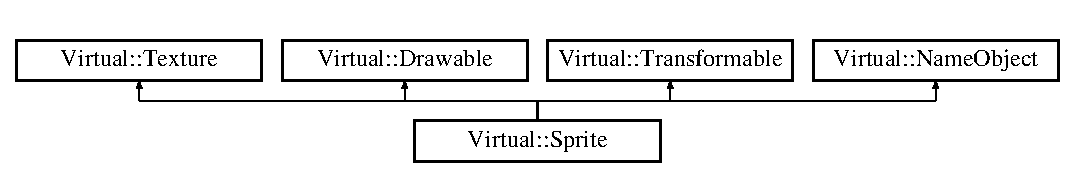
\includegraphics[height=3.000000cm]{class_virtual_1_1_sprite}
\end{center}
\end{figure}
\subsection*{Public Member Functions}
\begin{DoxyCompactItemize}
\item 
void \hyperlink{class_virtual_1_1_sprite_a57f581e0307ab2b2dd7c6922dba2a057}{draw} (S\+D\+L\+\_\+\+Renderer $\ast$renderer, \hyperlink{class_virtual_1_1_camera}{Camera} \&camera)
\begin{DoxyCompactList}\small\item\em Function that use engine to draw object. \end{DoxyCompactList}\end{DoxyCompactItemize}
\subsection*{Additional Inherited Members}


\subsection{Detailed Description}
Simple sprite class, like \hyperlink{class_virtual_1_1_label}{Label}. 

\subsection{Member Function Documentation}
\hypertarget{class_virtual_1_1_sprite_a57f581e0307ab2b2dd7c6922dba2a057}{}\label{class_virtual_1_1_sprite_a57f581e0307ab2b2dd7c6922dba2a057} 
\index{Virtual\+::\+Sprite@{Virtual\+::\+Sprite}!draw@{draw}}
\index{draw@{draw}!Virtual\+::\+Sprite@{Virtual\+::\+Sprite}}
\subsubsection{\texorpdfstring{draw()}{draw()}}
{\footnotesize\ttfamily void Virtual\+::\+Sprite\+::draw (\begin{DoxyParamCaption}\item[{S\+D\+L\+\_\+\+Renderer $\ast$}]{renderer,  }\item[{\hyperlink{class_virtual_1_1_camera}{Camera} \&}]{camera }\end{DoxyParamCaption})\hspace{0.3cm}{\ttfamily [virtual]}}



Function that use engine to draw object. 


\begin{DoxyParams}{Parameters}
{\em renderer} & -\/ pointer into S\+D\+L\+\_\+\+Renderer \\
\hline
{\em camera} & -\/ reference to camera in engine \\
\hline
\end{DoxyParams}


Implements \hyperlink{class_virtual_1_1_drawable_af7014800911efa59b96e538149e56f8b}{Virtual\+::\+Drawable}.



Reimplemented in \hyperlink{class_virtual_1_1_label_a077d7852f09f940a9932f63fb616351c}{Virtual\+::\+Label}.



The documentation for this class was generated from the following file\+:\begin{DoxyCompactItemize}
\item 
include/\+Virtual\+Eye/Render\+Utils.\+hpp\end{DoxyCompactItemize}

\hypertarget{class_virtual_1_1_texture}{}\section{Virtual\+:\+:Texture Class Reference}
\label{class_virtual_1_1_texture}\index{Virtual\+::\+Texture@{Virtual\+::\+Texture}}


Dynamic texture class, like \hyperlink{class_virtual_1_1_font}{Font}.  




{\ttfamily \#include $<$Render\+Utils.\+hpp$>$}

Inheritance diagram for Virtual\+:\+:Texture\+:\begin{figure}[H]
\begin{center}
\leavevmode
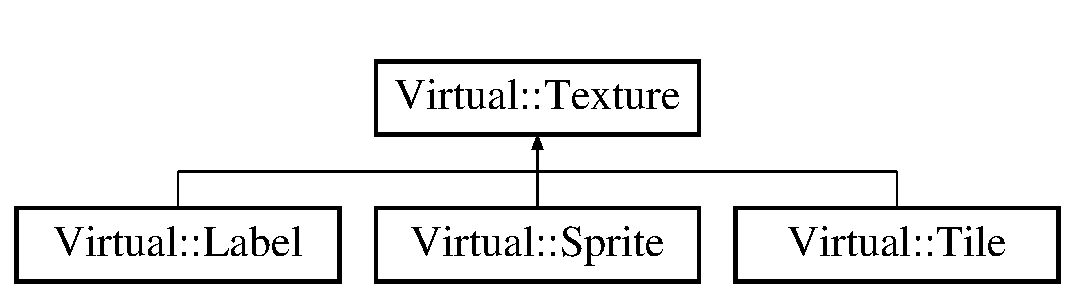
\includegraphics[height=3.000000cm]{class_virtual_1_1_texture}
\end{center}
\end{figure}
\subsection*{Public Member Functions}
\begin{DoxyCompactItemize}
\item 
void \hyperlink{class_virtual_1_1_texture_a8e0ffa6f92bfb5afab975a59f2b3b92f}{set\+Texture} (S\+D\+L\+\_\+\+Texture $\ast$texture)
\begin{DoxyCompactList}\small\item\em Dynamic texture class. \end{DoxyCompactList}\item 
S\+D\+L\+\_\+\+Texture $\ast$ \hyperlink{class_virtual_1_1_texture_a5c870d3c9b6db63922aa5cf451cd3422}{get\+Texture} ()
\end{DoxyCompactItemize}
\subsection*{Protected Attributes}
\begin{DoxyCompactItemize}
\item 
\hypertarget{class_virtual_1_1_texture_ae0101cbb0799e438722a16da7f25653a}{}\label{class_virtual_1_1_texture_ae0101cbb0799e438722a16da7f25653a} 
S\+D\+L\+\_\+\+Texture $\ast$ {\bfseries texture}
\end{DoxyCompactItemize}


\subsection{Detailed Description}
Dynamic texture class, like \hyperlink{class_virtual_1_1_font}{Font}. 

\subsection{Member Function Documentation}
\hypertarget{class_virtual_1_1_texture_a5c870d3c9b6db63922aa5cf451cd3422}{}\label{class_virtual_1_1_texture_a5c870d3c9b6db63922aa5cf451cd3422} 
\index{Virtual\+::\+Texture@{Virtual\+::\+Texture}!get\+Texture@{get\+Texture}}
\index{get\+Texture@{get\+Texture}!Virtual\+::\+Texture@{Virtual\+::\+Texture}}
\subsubsection{\texorpdfstring{get\+Texture()}{getTexture()}}
{\footnotesize\ttfamily S\+D\+L\+\_\+\+Texture$\ast$ Virtual\+::\+Texture\+::get\+Texture (\begin{DoxyParamCaption}{ }\end{DoxyParamCaption})}

\begin{DoxyReturn}{Returns}
S\+D\+L\+\_\+\+Texture pointer 
\end{DoxyReturn}
\hypertarget{class_virtual_1_1_texture_a8e0ffa6f92bfb5afab975a59f2b3b92f}{}\label{class_virtual_1_1_texture_a8e0ffa6f92bfb5afab975a59f2b3b92f} 
\index{Virtual\+::\+Texture@{Virtual\+::\+Texture}!set\+Texture@{set\+Texture}}
\index{set\+Texture@{set\+Texture}!Virtual\+::\+Texture@{Virtual\+::\+Texture}}
\subsubsection{\texorpdfstring{set\+Texture()}{setTexture()}}
{\footnotesize\ttfamily void Virtual\+::\+Texture\+::set\+Texture (\begin{DoxyParamCaption}\item[{S\+D\+L\+\_\+\+Texture $\ast$}]{texture }\end{DoxyParamCaption})}



Dynamic texture class. 


\begin{DoxyParams}{Parameters}
{\em texture} & -\/ pointer into S\+D\+L\+\_\+\+Texture viariable \\
\hline
\end{DoxyParams}


The documentation for this class was generated from the following file\+:\begin{DoxyCompactItemize}
\item 
include/\+Virtual\+Eye/Render\+Utils.\+hpp\end{DoxyCompactItemize}

\hypertarget{class_virtual_1_1_tile}{}\section{Virtual\+:\+:Tile Class Reference}
\label{class_virtual_1_1_tile}\index{Virtual\+::\+Tile@{Virtual\+::\+Tile}}


Simple tile class.  




{\ttfamily \#include $<$Render\+Utils.\+hpp$>$}

Inheritance diagram for Virtual\+:\+:Tile\+:\begin{figure}[H]
\begin{center}
\leavevmode
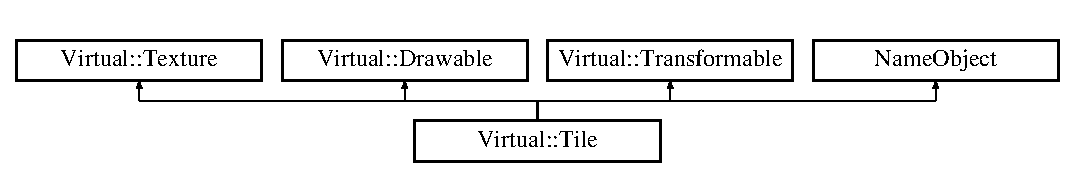
\includegraphics[height=3.000000cm]{class_virtual_1_1_tile}
\end{center}
\end{figure}
\subsection*{Public Member Functions}
\begin{DoxyCompactItemize}
\item 
void \hyperlink{class_virtual_1_1_tile_a7e275a90e1b528130445c8e053d4dc66}{set\+Tile} (int type)
\begin{DoxyCompactList}\small\item\em Sets tile type number. \end{DoxyCompactList}\item 
int \hyperlink{class_virtual_1_1_tile_ae535b36cb182c5376739a4d6cdb7306b}{get\+Tile} ()
\end{DoxyCompactItemize}
\subsection*{Additional Inherited Members}


\subsection{Detailed Description}
Simple tile class. 

\subsection{Member Function Documentation}
\hypertarget{class_virtual_1_1_tile_ae535b36cb182c5376739a4d6cdb7306b}{}\label{class_virtual_1_1_tile_ae535b36cb182c5376739a4d6cdb7306b} 
\index{Virtual\+::\+Tile@{Virtual\+::\+Tile}!get\+Tile@{get\+Tile}}
\index{get\+Tile@{get\+Tile}!Virtual\+::\+Tile@{Virtual\+::\+Tile}}
\subsubsection{\texorpdfstring{get\+Tile()}{getTile()}}
{\footnotesize\ttfamily int Virtual\+::\+Tile\+::get\+Tile (\begin{DoxyParamCaption}{ }\end{DoxyParamCaption})}

\begin{DoxyReturn}{Returns}
integer tile type number 
\end{DoxyReturn}
\hypertarget{class_virtual_1_1_tile_a7e275a90e1b528130445c8e053d4dc66}{}\label{class_virtual_1_1_tile_a7e275a90e1b528130445c8e053d4dc66} 
\index{Virtual\+::\+Tile@{Virtual\+::\+Tile}!set\+Tile@{set\+Tile}}
\index{set\+Tile@{set\+Tile}!Virtual\+::\+Tile@{Virtual\+::\+Tile}}
\subsubsection{\texorpdfstring{set\+Tile()}{setTile()}}
{\footnotesize\ttfamily void Virtual\+::\+Tile\+::set\+Tile (\begin{DoxyParamCaption}\item[{int}]{type }\end{DoxyParamCaption})}



Sets tile type number. 


\begin{DoxyParams}{Parameters}
{\em type} & -\/ number of type \\
\hline
\end{DoxyParams}


The documentation for this class was generated from the following file\+:\begin{DoxyCompactItemize}
\item 
include/\+Virtual\+Eye/Render\+Utils.\+hpp\end{DoxyCompactItemize}

\hypertarget{class_virtual_1_1_transformable}{}\section{Virtual\+:\+:Transformable Class Reference}
\label{class_virtual_1_1_transformable}\index{Virtual\+::\+Transformable@{Virtual\+::\+Transformable}}


Class to manupulate position and size of object.  




{\ttfamily \#include $<$Transformable.\+hpp$>$}

Inheritance diagram for Virtual\+:\+:Transformable\+:\begin{figure}[H]
\begin{center}
\leavevmode
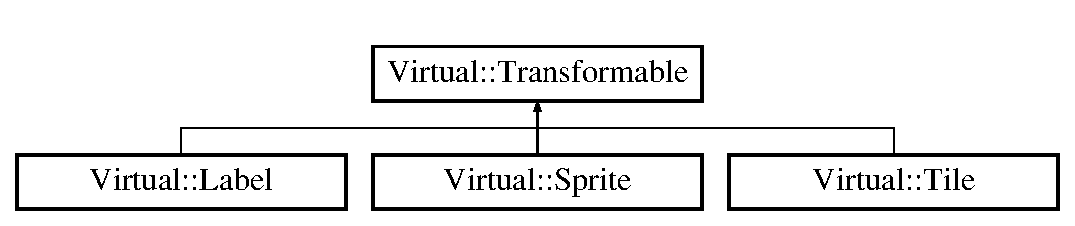
\includegraphics[height=2.000000cm]{class_virtual_1_1_transformable}
\end{center}
\end{figure}
\subsection*{Public Member Functions}
\begin{DoxyCompactItemize}
\item 
\hyperlink{struct_virtual_1_1_vector2}{Vector2}$<$ int $>$ \hyperlink{class_virtual_1_1_transformable_a2bb830f06c5123ae69d0584eef5f16f3}{get\+Position} ()
\item 
\hyperlink{struct_virtual_1_1_vector2}{Vector2}$<$ int $>$ \hyperlink{class_virtual_1_1_transformable_a816bf127c89675265776e94ef849e6e8}{get\+Parametres} ()
\item 
\hyperlink{struct_virtual_1_1_vector2}{Vector2}$<$ int $>$ \hyperlink{class_virtual_1_1_transformable_adbccc4539561975b0de4471d05ca7541}{get\+Crop\+Position} ()
\item 
\hyperlink{struct_virtual_1_1_vector2}{Vector2}$<$ int $>$ \hyperlink{class_virtual_1_1_transformable_a22aa918ae175dea89c27728a20c29f82}{get\+Crop\+Parametres} ()
\item 
\hyperlink{struct_virtual_1_1_rectangle}{Rectangle}$<$ int $>$ \hyperlink{class_virtual_1_1_transformable_aa25efa18322fe9eaa187cd7cb54909ae}{get\+Rectangle} ()
\item 
int \hyperlink{class_virtual_1_1_transformable_acda950f2b5d3f2b85aec5663bec79611}{get\+Angle} ()
\item 
\hyperlink{struct_virtual_1_1_vector2}{Vector2}$<$ int $>$ \hyperlink{class_virtual_1_1_transformable_a703da601d8ef871a03b0da591edda2fe}{get\+Center} ()
\item 
void \hyperlink{class_virtual_1_1_transformable_a2c1168cb1d892fbddd978c7d45dfcba9}{set\+Position} (\hyperlink{struct_virtual_1_1_vector2}{Vector2}$<$ int $>$ position)
\begin{DoxyCompactList}\small\item\em Setting position of object. \end{DoxyCompactList}\item 
void \hyperlink{class_virtual_1_1_transformable_a67d42e58b8f2fc45b565aa51e3f29f67}{set\+Parametres} (\hyperlink{struct_virtual_1_1_vector2}{Vector2}$<$ int $>$ size)
\begin{DoxyCompactList}\small\item\em Setting size of object. \end{DoxyCompactList}\item 
void \hyperlink{class_virtual_1_1_transformable_afa2e1b7971db9c916a38f7dfa06a0b26}{set\+Crop\+Position} (\hyperlink{struct_virtual_1_1_vector2}{Vector2}$<$ int $>$ crop\+Position)
\begin{DoxyCompactList}\small\item\em Setting position of crop of texture. \end{DoxyCompactList}\item 
void \hyperlink{class_virtual_1_1_transformable_a558026b1336c4f24c2bc70debc01800c}{set\+Crop\+Parametres} (\hyperlink{struct_virtual_1_1_vector2}{Vector2}$<$ int $>$ crop\+Size)
\begin{DoxyCompactList}\small\item\em Setting position of crop of texture. \end{DoxyCompactList}\item 
void \hyperlink{class_virtual_1_1_transformable_ad86a98728222a2b879afa41ba27dfc58}{set\+Rectangle} (\hyperlink{struct_virtual_1_1_rectangle}{Rectangle}$<$ int $>$ rect)
\begin{DoxyCompactList}\small\item\em Setting position and size of sprite. \end{DoxyCompactList}\item 
void \hyperlink{class_virtual_1_1_transformable_ae7305c3fe8a7bd9f4a1138a9d097bfab}{set\+Angle} (int angle)
\begin{DoxyCompactList}\small\item\em Setting angle of sprite. \end{DoxyCompactList}\item 
void \hyperlink{class_virtual_1_1_transformable_a4d0e9c61931af6b42fac1dc0c3a1ed21}{set\+Flip} (S\+D\+L\+\_\+\+Renderer\+Flip flip)
\begin{DoxyCompactList}\small\item\em Setting flip of texture. \end{DoxyCompactList}\item 
void \hyperlink{class_virtual_1_1_transformable_a80eb3848090682f3ad3bd3faf879f6ab}{move} (\hyperlink{struct_virtual_1_1_vector2}{Vector2}$<$ int $>$ relative\+Position, double delta)
\begin{DoxyCompactList}\small\item\em Setting flip of texture. \end{DoxyCompactList}\item 
\hypertarget{class_virtual_1_1_transformable_a997867ac2fabb95a7244caeeb26d8b05}{}\label{class_virtual_1_1_transformable_a997867ac2fabb95a7244caeeb26d8b05} 
bool {\bfseries is\+Collide} (\hyperlink{class_virtual_1_1_transformable}{Transformable} \&)
\end{DoxyCompactItemize}
\subsection*{Protected Attributes}
\begin{DoxyCompactItemize}
\item 
\hypertarget{class_virtual_1_1_transformable_af218a7ebdc91c7714b791a5973c3ff43}{}\label{class_virtual_1_1_transformable_af218a7ebdc91c7714b791a5973c3ff43} 
S\+D\+L\+\_\+\+Rect {\bfseries rect}
\item 
\hypertarget{class_virtual_1_1_transformable_a38b781918dcf60c7154f0a288c5bb434}{}\label{class_virtual_1_1_transformable_a38b781918dcf60c7154f0a288c5bb434} 
S\+D\+L\+\_\+\+Rect {\bfseries crop\+Rect}
\item 
\hypertarget{class_virtual_1_1_transformable_aca6c8a4c255cc8dc72bf831cbeb918bb}{}\label{class_virtual_1_1_transformable_aca6c8a4c255cc8dc72bf831cbeb918bb} 
S\+D\+L\+\_\+\+Renderer\+Flip {\bfseries flip}
\item 
\hypertarget{class_virtual_1_1_transformable_a6ce7c408bf4fc4b21147dce206a7bb29}{}\label{class_virtual_1_1_transformable_a6ce7c408bf4fc4b21147dce206a7bb29} 
int {\bfseries angle}
\end{DoxyCompactItemize}


\subsection{Detailed Description}
Class to manupulate position and size of object. 

\subsection{Member Function Documentation}
\hypertarget{class_virtual_1_1_transformable_acda950f2b5d3f2b85aec5663bec79611}{}\label{class_virtual_1_1_transformable_acda950f2b5d3f2b85aec5663bec79611} 
\index{Virtual\+::\+Transformable@{Virtual\+::\+Transformable}!get\+Angle@{get\+Angle}}
\index{get\+Angle@{get\+Angle}!Virtual\+::\+Transformable@{Virtual\+::\+Transformable}}
\subsubsection{\texorpdfstring{get\+Angle()}{getAngle()}}
{\footnotesize\ttfamily int Virtual\+::\+Transformable\+::get\+Angle (\begin{DoxyParamCaption}{ }\end{DoxyParamCaption})}

\begin{DoxyReturn}{Returns}
angle of object 
\end{DoxyReturn}
\hypertarget{class_virtual_1_1_transformable_a703da601d8ef871a03b0da591edda2fe}{}\label{class_virtual_1_1_transformable_a703da601d8ef871a03b0da591edda2fe} 
\index{Virtual\+::\+Transformable@{Virtual\+::\+Transformable}!get\+Center@{get\+Center}}
\index{get\+Center@{get\+Center}!Virtual\+::\+Transformable@{Virtual\+::\+Transformable}}
\subsubsection{\texorpdfstring{get\+Center()}{getCenter()}}
{\footnotesize\ttfamily \hyperlink{struct_virtual_1_1_vector2}{Vector2}$<$int$>$ Virtual\+::\+Transformable\+::get\+Center (\begin{DoxyParamCaption}{ }\end{DoxyParamCaption})}

\begin{DoxyReturn}{Returns}
center of texture 
\end{DoxyReturn}
\hypertarget{class_virtual_1_1_transformable_a22aa918ae175dea89c27728a20c29f82}{}\label{class_virtual_1_1_transformable_a22aa918ae175dea89c27728a20c29f82} 
\index{Virtual\+::\+Transformable@{Virtual\+::\+Transformable}!get\+Crop\+Parametres@{get\+Crop\+Parametres}}
\index{get\+Crop\+Parametres@{get\+Crop\+Parametres}!Virtual\+::\+Transformable@{Virtual\+::\+Transformable}}
\subsubsection{\texorpdfstring{get\+Crop\+Parametres()}{getCropParametres()}}
{\footnotesize\ttfamily \hyperlink{struct_virtual_1_1_vector2}{Vector2}$<$int$>$ Virtual\+::\+Transformable\+::get\+Crop\+Parametres (\begin{DoxyParamCaption}{ }\end{DoxyParamCaption})}

\begin{DoxyReturn}{Returns}
size of texture crop in object 
\end{DoxyReturn}
\hypertarget{class_virtual_1_1_transformable_adbccc4539561975b0de4471d05ca7541}{}\label{class_virtual_1_1_transformable_adbccc4539561975b0de4471d05ca7541} 
\index{Virtual\+::\+Transformable@{Virtual\+::\+Transformable}!get\+Crop\+Position@{get\+Crop\+Position}}
\index{get\+Crop\+Position@{get\+Crop\+Position}!Virtual\+::\+Transformable@{Virtual\+::\+Transformable}}
\subsubsection{\texorpdfstring{get\+Crop\+Position()}{getCropPosition()}}
{\footnotesize\ttfamily \hyperlink{struct_virtual_1_1_vector2}{Vector2}$<$int$>$ Virtual\+::\+Transformable\+::get\+Crop\+Position (\begin{DoxyParamCaption}{ }\end{DoxyParamCaption})}

\begin{DoxyReturn}{Returns}
position of texture crop in object 
\end{DoxyReturn}
\hypertarget{class_virtual_1_1_transformable_a816bf127c89675265776e94ef849e6e8}{}\label{class_virtual_1_1_transformable_a816bf127c89675265776e94ef849e6e8} 
\index{Virtual\+::\+Transformable@{Virtual\+::\+Transformable}!get\+Parametres@{get\+Parametres}}
\index{get\+Parametres@{get\+Parametres}!Virtual\+::\+Transformable@{Virtual\+::\+Transformable}}
\subsubsection{\texorpdfstring{get\+Parametres()}{getParametres()}}
{\footnotesize\ttfamily \hyperlink{struct_virtual_1_1_vector2}{Vector2}$<$int$>$ Virtual\+::\+Transformable\+::get\+Parametres (\begin{DoxyParamCaption}{ }\end{DoxyParamCaption})}

\begin{DoxyReturn}{Returns}
size of object 
\end{DoxyReturn}
\hypertarget{class_virtual_1_1_transformable_a2bb830f06c5123ae69d0584eef5f16f3}{}\label{class_virtual_1_1_transformable_a2bb830f06c5123ae69d0584eef5f16f3} 
\index{Virtual\+::\+Transformable@{Virtual\+::\+Transformable}!get\+Position@{get\+Position}}
\index{get\+Position@{get\+Position}!Virtual\+::\+Transformable@{Virtual\+::\+Transformable}}
\subsubsection{\texorpdfstring{get\+Position()}{getPosition()}}
{\footnotesize\ttfamily \hyperlink{struct_virtual_1_1_vector2}{Vector2}$<$int$>$ Virtual\+::\+Transformable\+::get\+Position (\begin{DoxyParamCaption}{ }\end{DoxyParamCaption})}

\begin{DoxyReturn}{Returns}
position of object 
\end{DoxyReturn}
\hypertarget{class_virtual_1_1_transformable_aa25efa18322fe9eaa187cd7cb54909ae}{}\label{class_virtual_1_1_transformable_aa25efa18322fe9eaa187cd7cb54909ae} 
\index{Virtual\+::\+Transformable@{Virtual\+::\+Transformable}!get\+Rectangle@{get\+Rectangle}}
\index{get\+Rectangle@{get\+Rectangle}!Virtual\+::\+Transformable@{Virtual\+::\+Transformable}}
\subsubsection{\texorpdfstring{get\+Rectangle()}{getRectangle()}}
{\footnotesize\ttfamily \hyperlink{struct_virtual_1_1_rectangle}{Rectangle}$<$int$>$ Virtual\+::\+Transformable\+::get\+Rectangle (\begin{DoxyParamCaption}{ }\end{DoxyParamCaption})}

\begin{DoxyReturn}{Returns}
size of texture crop in object 
\end{DoxyReturn}
\hypertarget{class_virtual_1_1_transformable_a80eb3848090682f3ad3bd3faf879f6ab}{}\label{class_virtual_1_1_transformable_a80eb3848090682f3ad3bd3faf879f6ab} 
\index{Virtual\+::\+Transformable@{Virtual\+::\+Transformable}!move@{move}}
\index{move@{move}!Virtual\+::\+Transformable@{Virtual\+::\+Transformable}}
\subsubsection{\texorpdfstring{move()}{move()}}
{\footnotesize\ttfamily void Virtual\+::\+Transformable\+::move (\begin{DoxyParamCaption}\item[{\hyperlink{struct_virtual_1_1_vector2}{Vector2}$<$ int $>$}]{relative\+Position,  }\item[{double}]{delta }\end{DoxyParamCaption})}



Setting flip of texture. 


\begin{DoxyParams}{Parameters}
{\em flip} & -\/ for exaple (F\+L\+I\+P(\+N\+O\+N\+E)) \\
\hline
\end{DoxyParams}
\hypertarget{class_virtual_1_1_transformable_ae7305c3fe8a7bd9f4a1138a9d097bfab}{}\label{class_virtual_1_1_transformable_ae7305c3fe8a7bd9f4a1138a9d097bfab} 
\index{Virtual\+::\+Transformable@{Virtual\+::\+Transformable}!set\+Angle@{set\+Angle}}
\index{set\+Angle@{set\+Angle}!Virtual\+::\+Transformable@{Virtual\+::\+Transformable}}
\subsubsection{\texorpdfstring{set\+Angle()}{setAngle()}}
{\footnotesize\ttfamily void Virtual\+::\+Transformable\+::set\+Angle (\begin{DoxyParamCaption}\item[{int}]{angle }\end{DoxyParamCaption})}



Setting angle of sprite. 


\begin{DoxyParams}{Parameters}
{\em angle} & -\/ angle in degrees \\
\hline
\end{DoxyParams}
\hypertarget{class_virtual_1_1_transformable_a558026b1336c4f24c2bc70debc01800c}{}\label{class_virtual_1_1_transformable_a558026b1336c4f24c2bc70debc01800c} 
\index{Virtual\+::\+Transformable@{Virtual\+::\+Transformable}!set\+Crop\+Parametres@{set\+Crop\+Parametres}}
\index{set\+Crop\+Parametres@{set\+Crop\+Parametres}!Virtual\+::\+Transformable@{Virtual\+::\+Transformable}}
\subsubsection{\texorpdfstring{set\+Crop\+Parametres()}{setCropParametres()}}
{\footnotesize\ttfamily void Virtual\+::\+Transformable\+::set\+Crop\+Parametres (\begin{DoxyParamCaption}\item[{\hyperlink{struct_virtual_1_1_vector2}{Vector2}$<$ int $>$}]{crop\+Size }\end{DoxyParamCaption})}



Setting position of crop of texture. 


\begin{DoxyParams}{Parameters}
{\em crop\+Size} & -\/ coords of crop position(width and height) \\
\hline
\end{DoxyParams}
\hypertarget{class_virtual_1_1_transformable_afa2e1b7971db9c916a38f7dfa06a0b26}{}\label{class_virtual_1_1_transformable_afa2e1b7971db9c916a38f7dfa06a0b26} 
\index{Virtual\+::\+Transformable@{Virtual\+::\+Transformable}!set\+Crop\+Position@{set\+Crop\+Position}}
\index{set\+Crop\+Position@{set\+Crop\+Position}!Virtual\+::\+Transformable@{Virtual\+::\+Transformable}}
\subsubsection{\texorpdfstring{set\+Crop\+Position()}{setCropPosition()}}
{\footnotesize\ttfamily void Virtual\+::\+Transformable\+::set\+Crop\+Position (\begin{DoxyParamCaption}\item[{\hyperlink{struct_virtual_1_1_vector2}{Vector2}$<$ int $>$}]{crop\+Position }\end{DoxyParamCaption})}



Setting position of crop of texture. 


\begin{DoxyParams}{Parameters}
{\em crop\+Position} & -\/ coords of crop position(x and y) \\
\hline
\end{DoxyParams}
\hypertarget{class_virtual_1_1_transformable_a4d0e9c61931af6b42fac1dc0c3a1ed21}{}\label{class_virtual_1_1_transformable_a4d0e9c61931af6b42fac1dc0c3a1ed21} 
\index{Virtual\+::\+Transformable@{Virtual\+::\+Transformable}!set\+Flip@{set\+Flip}}
\index{set\+Flip@{set\+Flip}!Virtual\+::\+Transformable@{Virtual\+::\+Transformable}}
\subsubsection{\texorpdfstring{set\+Flip()}{setFlip()}}
{\footnotesize\ttfamily void Virtual\+::\+Transformable\+::set\+Flip (\begin{DoxyParamCaption}\item[{S\+D\+L\+\_\+\+Renderer\+Flip}]{flip }\end{DoxyParamCaption})}



Setting flip of texture. 


\begin{DoxyParams}{Parameters}
{\em flip} & -\/ for exaple (F\+L\+I\+P(\+N\+O\+N\+E)) \\
\hline
\end{DoxyParams}
\hypertarget{class_virtual_1_1_transformable_a67d42e58b8f2fc45b565aa51e3f29f67}{}\label{class_virtual_1_1_transformable_a67d42e58b8f2fc45b565aa51e3f29f67} 
\index{Virtual\+::\+Transformable@{Virtual\+::\+Transformable}!set\+Parametres@{set\+Parametres}}
\index{set\+Parametres@{set\+Parametres}!Virtual\+::\+Transformable@{Virtual\+::\+Transformable}}
\subsubsection{\texorpdfstring{set\+Parametres()}{setParametres()}}
{\footnotesize\ttfamily void Virtual\+::\+Transformable\+::set\+Parametres (\begin{DoxyParamCaption}\item[{\hyperlink{struct_virtual_1_1_vector2}{Vector2}$<$ int $>$}]{size }\end{DoxyParamCaption})}



Setting size of object. 


\begin{DoxyParams}{Parameters}
{\em size} & -\/ coords of position \\
\hline
\end{DoxyParams}
\hypertarget{class_virtual_1_1_transformable_a2c1168cb1d892fbddd978c7d45dfcba9}{}\label{class_virtual_1_1_transformable_a2c1168cb1d892fbddd978c7d45dfcba9} 
\index{Virtual\+::\+Transformable@{Virtual\+::\+Transformable}!set\+Position@{set\+Position}}
\index{set\+Position@{set\+Position}!Virtual\+::\+Transformable@{Virtual\+::\+Transformable}}
\subsubsection{\texorpdfstring{set\+Position()}{setPosition()}}
{\footnotesize\ttfamily void Virtual\+::\+Transformable\+::set\+Position (\begin{DoxyParamCaption}\item[{\hyperlink{struct_virtual_1_1_vector2}{Vector2}$<$ int $>$}]{position }\end{DoxyParamCaption})}



Setting position of object. 


\begin{DoxyParams}{Parameters}
{\em position} & -\/ coords of position \\
\hline
\end{DoxyParams}
\hypertarget{class_virtual_1_1_transformable_ad86a98728222a2b879afa41ba27dfc58}{}\label{class_virtual_1_1_transformable_ad86a98728222a2b879afa41ba27dfc58} 
\index{Virtual\+::\+Transformable@{Virtual\+::\+Transformable}!set\+Rectangle@{set\+Rectangle}}
\index{set\+Rectangle@{set\+Rectangle}!Virtual\+::\+Transformable@{Virtual\+::\+Transformable}}
\subsubsection{\texorpdfstring{set\+Rectangle()}{setRectangle()}}
{\footnotesize\ttfamily void Virtual\+::\+Transformable\+::set\+Rectangle (\begin{DoxyParamCaption}\item[{\hyperlink{struct_virtual_1_1_rectangle}{Rectangle}$<$ int $>$}]{rect }\end{DoxyParamCaption})}



Setting position and size of sprite. 


\begin{DoxyParams}{Parameters}
{\em rect} & -\/ coords of position and width and height \\
\hline
\end{DoxyParams}


The documentation for this class was generated from the following file\+:\begin{DoxyCompactItemize}
\item 
include/\+Virtual\+Eye/Transformable.\+hpp\end{DoxyCompactItemize}

\hypertarget{struct_virtual_1_1_vector2}{}\section{Virtual\+:\+:Vector2$<$ T $>$ Struct Template Reference}
\label{struct_virtual_1_1_vector2}\index{Virtual\+::\+Vector2$<$ T $>$@{Virtual\+::\+Vector2$<$ T $>$}}


The simple coorinates of one point on the screen.  




{\ttfamily \#include $<$Math.\+hpp$>$}

\subsection*{Public Member Functions}
\begin{DoxyCompactItemize}
\item 
\hyperlink{struct_virtual_1_1_vector2_add372f623a2a5c19f1f20f491cf7001c}{Vector2} ()
\begin{DoxyCompactList}\small\item\em Default zero constructor. \end{DoxyCompactList}\item 
\hyperlink{struct_virtual_1_1_vector2_a5debf297b5880d21e4ee0748dc620160}{Vector2} (T xx, T yy)
\begin{DoxyCompactList}\small\item\em Default custom constructor. \end{DoxyCompactList}\end{DoxyCompactItemize}
\subsection*{Public Attributes}
\begin{DoxyCompactItemize}
\item 
\hypertarget{struct_virtual_1_1_vector2_a919a8ee5d1a3cdd8bddef88b02892cda}{}\label{struct_virtual_1_1_vector2_a919a8ee5d1a3cdd8bddef88b02892cda} 
T {\bfseries x}
\item 
\hypertarget{struct_virtual_1_1_vector2_a88e297ba93191d0d797a0c32c1f08d0f}{}\label{struct_virtual_1_1_vector2_a88e297ba93191d0d797a0c32c1f08d0f} 
T {\bfseries y}
\end{DoxyCompactItemize}


\subsection{Detailed Description}
\subsubsection*{template$<$typename T$>$\newline
struct Virtual\+::\+Vector2$<$ T $>$}

The simple coorinates of one point on the screen. 

\subsection{Constructor \& Destructor Documentation}
\hypertarget{struct_virtual_1_1_vector2_add372f623a2a5c19f1f20f491cf7001c}{}\label{struct_virtual_1_1_vector2_add372f623a2a5c19f1f20f491cf7001c} 
\index{Virtual\+::\+Vector2@{Virtual\+::\+Vector2}!Vector2@{Vector2}}
\index{Vector2@{Vector2}!Virtual\+::\+Vector2@{Virtual\+::\+Vector2}}
\subsubsection{\texorpdfstring{Vector2()}{Vector2()}\hspace{0.1cm}{\footnotesize\ttfamily [1/2]}}
{\footnotesize\ttfamily template$<$typename T$>$ \\
\hyperlink{struct_virtual_1_1_vector2}{Virtual\+::\+Vector2}$<$ T $>$\+::\hyperlink{struct_virtual_1_1_vector2}{Vector2} (\begin{DoxyParamCaption}{ }\end{DoxyParamCaption})\hspace{0.3cm}{\ttfamily [inline]}}



Default zero constructor. 

This constructor append of each variables zero. \hypertarget{struct_virtual_1_1_vector2_a5debf297b5880d21e4ee0748dc620160}{}\label{struct_virtual_1_1_vector2_a5debf297b5880d21e4ee0748dc620160} 
\index{Virtual\+::\+Vector2@{Virtual\+::\+Vector2}!Vector2@{Vector2}}
\index{Vector2@{Vector2}!Virtual\+::\+Vector2@{Virtual\+::\+Vector2}}
\subsubsection{\texorpdfstring{Vector2()}{Vector2()}\hspace{0.1cm}{\footnotesize\ttfamily [2/2]}}
{\footnotesize\ttfamily template$<$typename T$>$ \\
\hyperlink{struct_virtual_1_1_vector2}{Virtual\+::\+Vector2}$<$ T $>$\+::\hyperlink{struct_virtual_1_1_vector2}{Vector2} (\begin{DoxyParamCaption}\item[{T}]{xx,  }\item[{T}]{yy }\end{DoxyParamCaption})\hspace{0.3cm}{\ttfamily [inline]}}



Default custom constructor. 


\begin{DoxyParams}{Parameters}
{\em xx} & -\/ x value \\
\hline
{\em yy} & -\/ y value\\
\hline
\end{DoxyParams}
This constructor append of each variables given values. 

The documentation for this struct was generated from the following file\+:\begin{DoxyCompactItemize}
\item 
include/\+Virtual\+Eye/Math.\+hpp\end{DoxyCompactItemize}

%--- End generated contents ---

% Index
\backmatter
\newpage
\phantomsection
\clearemptydoublepage
\addcontentsline{toc}{chapter}{Index}
\printindex

\end{document}
